\documentclass[conference,compsoc]{IEEEtran}

% This is because IEEE is a bad latex style
\newtheorem{definition}{Definition}
\newtheorem{lemma}{Lemma}
\newtheorem{proof}{Proof}
% \documentclass[sigconf, anonymous]{acmart}

% \usepackage{usenix-2020-09}

\usepackage{enumitem}
\usepackage{arydshln}
% \usepackage{amsthm}
\usepackage{amssymb}
\usepackage{subcaption}
% \usepackage{subfig}
\usepackage{subcaption}
\usepackage{graphicx}
\usepackage{amsmath}
\usepackage{url}
\usepackage{color}
\usepackage{booktabs}
\usepackage{multirow}
\usepackage{algorithm}
\usepackage{algpseudocode, float}
\usepackage{bbding}
\usepackage{bbding}
\usepackage{tikz}
\usetikzlibrary{shapes.geometric,arrows,decorations.markings, arrows.meta}
\usetikzlibrary{positioning, calc}


\usepackage{forest}

\usetikzlibrary{graphs}
\usetikzlibrary{arrows,automata}

\forestset{%
angle below/.style={
tikz+={%
\draw ($(!1.child anchor)!.25!(.parent anchor)$) [bend right=15] to ($(.parent anchor)!.75!(!l.child anchor)$);
},
},
small angle below/.style={
tikz+={%
\draw ($(!1.child anchor)!.5!(.parent anchor)$) [bend right=15] to ($(.parent anchor)!.5!(!l.child anchor)$);
},
},
arrow below/.style={
tikz+={%
\draw[->] ($(!1.child anchor)!.30!(.parent anchor)$) [bend right=20] to ($(.parent anchor)!.7!(!l.child anchor)$);
},
},
}




% \raggedbottom
% 
\pagestyle{plain}
\begin{document}


\title{Attack Tree Distance: a practical examination of tree difference measurement within cyber security}

\iffalse{
    \author{Nathan D. Schiele}
    \orcid{0000-0003-1186-1503}
    \affiliation{\institution{Leiden University}
        \city{Leiden}
        \country{The Netherlands}}
    \email{n.d.schiele@liacs.leidenuniv.nl}


    \author{Olga Gadyatskaya}
    \orcid{0000-0002-3760-9165}
    \affiliation{\institution{Leiden University}
        \city{Leiden}
        \country{The Netherlands}}
    \email{o.gadyatskaya@liacs.leidenuniv.nl}
}\fi
\author{Anonymized for submission}




% \acmConference[ACSAC]{ACSAC}
% \acmYear{2024}
% \acmBooktitle{Proceedings of the 32nd ACM Symposium on the Foundations of Software Engineering (FSE '24), November 15--19, 2024, Porto de Galinhas, Brazil}
% \acmBooktitle{Submission to ACSAC'24}

% \settopmatter{printfolios=true}

% \begin{teaserfigure}
%     \includegraphics[width=\textwidth]{img/Teaser02}
%     \caption{Participant created ADT}
%     \Description{A collage of ADTs that were created by participants}
%     \end{teaserfigure}

% \begin{teaserfigure}
% \includegraphics[width=\textwidth]{img/CollageTeaser}
% \caption{Assorted participant created ADTs}
% \Description{A collage of ADTs that were created by participants}
% \end{teaserfigure}




\maketitle              % typeset the header of the contribution
\newcommand{\OG}[1]{{\color{blue} OG: #1}}
\newcommand{\NS}[1]{{\color{purple} NS: #1}}

\newcommand{\etal}{et al.}
\newcommand{\id}[2]{#1-#2}
\newcommand{\hypothesis}[1]{$\text{H}_\text{#1}$}
\newcommand{\RQ}[1]{\textbf{RQ#1}}

\newcommand{\ICS}{NCS}
\newcommand{\SEC}{CS}



\newcommand{\AND}{AND}
\newcommand{\SAND}{SAND}
\newcommand{\OR}    {OR}

\newcommand{\childFunc}[1]{\text{child}({#1})}
\newcommand{\parentFunc}[1]{\text{par}({#1})}

\newcommand{\ATnode}[2]{t_{{#1}.{#2}}}
\newcommand{\ATlabel}[2]{l_{{#1}.{#2}}}

\newcommand{\hResponse}[1]{\texttt{#1} - }

\newcommand{\anonfoot}{\footnote{Anonymized for submission}}


\newcommand{\qIndent}{4em}
\newcommand{\qsIndent}{2em}
\newcommand{\surveyq}[1]{\textbf{#1:}}





% \begin{abstract}
%     \absSection{Context} Attack trees are a recommended threat modeling method, but there is no established approach to compare them. \\
% \absSection{Objective} We aim to analyze varied distance metrics which are capable of comparing attack tree models produced by human experts, based on both the structure of the tree itself and the meaning of the node labels.\\
%     \absSection{Method} We elicit a set of requirements for attack tree distance measures following from the theoretical underpinning of the model and the usability needs of human experts. We propose a repeatable method of experimental attack tree distance measures validation. To collect a dataset of attack trees that can be used for evaluation and comparison of the measures, we design and execute a human study ($n=39$). We then define four attack tree distance measures (three novel and one established) and compare them on the dataset. \\
% \absSection{Results} From our experimental results, we find that applying semantic similarity as a means of comparing node labels is a valid approach. Further, we find that the tree edit distance (established) and the radical distance (novel) are the most promising methods of comparison in most circumstances.\\
%     \absSection{Conclusion} Our results suggest that these two methods can be used to compare real-world attack trees and to identify similar attack trees. Future research can focus on assessing other metrics based on established attack tree semantics. 
% \end{abstract}

\begin{abstract}
Attack trees are a recommended threat modeling method, but there is no established approach to compare them. In practice, there is often a need of comparing attack tree models produced by human experts, based on both the structure of the tree and the meaning of the node labels. In this work, we investigate the problem of comparing attack trees and measuring their similarity. We elicit a set of requirements for attack tree distance measures following from the theoretical underpinning of the model and the usability needs of human experts. We propose a repeatable method of experimental attack tree distance measures validation. To collect a dataset of attack trees that can be used for evaluation and comparison of the measures, we design and execute a human study ($n=39$). We then define four attack tree distance measures (three novel and one established) and compare them on the dataset. 

From our experimental results, we find that applying semantic similarity as a means of comparing node labels is a valid approach. Further, we find that the tree edit distance (established) and the radical distance (novel) are the most promising methods of measuring attack tree similarity in most circumstances. Our results suggest that these two methods can be used to identify similar real-world attack trees. We also outline future research directions that can focus on assessing other metrics based on established attack tree semantics.
\end{abstract}





\section{Introduction}
\label{sec:introduction}

Threat modeling seeks to organize threat information that aids in comprehension and analysis of cyber attacks~\cite{andersonSecurityEngineeringGuide2020,schneierSecretsLiesDigital2000}. \emph{Attack trees} are a popular method for threat modeling in software engineering~\cite{shostack2014threat,tarandach2020threat}, security requirements elicitation~\cite{rashid2016discovering,mai2018modeling}, and security risk assessment~\cite{ingoldsby2010attack,paul2014unifying}. There is a rich literature on attack tree models designed by experts in order to better understand threats to a particular system, e.g., ATMs~\cite{fraile2016using}, smart cars~\cite{kong2018security,ren2011novel}, cloud systems~\cite{wang2012threat,duncan2019combined}, smart grids~\cite{beckers2014determining,mclaughlin2010energy}, medical implants~\cite{siddiqi2018attack} or SCADA systems~\cite{ten2007vulnerability}. Furthermore, in the past few years, there has been a growing interest in the automated synthesis of attack trees using formal system models~\cite{widel2019beyond,ivanova2015attack,vigo2014automated,pinchinat2015atsyra,gadyatskayaRefinementAwareGenerationAttack2017}, libraries of attack patterns~\cite{jhawar2018semi,bryans2020template}, or even machine learning methods~\cite{sowka2021towards} and most recently large language models (LLMs)~\cite{gadyatskaya2023chatgpt}.

Given this proliferation of attack tree models produced for different scenarios, especially when they are synthesized automatically, novel questions emerge. For example, one might wonder \emph{how can we establish whether two attack trees produced by different experts describe similar attack scenarios}. 
Another question, posed in~\cite{gadyatskaya2023chatgpt}, relates to establishing the quality of an automatically synthesized attack tree by comparing it to a tree designed by a human expert. However, currently, there is no standard method for comparing attack trees or measuring their similarity. Existing attack tree semantics can partially answer this question as semantics provide a way to define the meaning of an attack tree model~\cite{mauwFoundationsAttackTrees2006}. Yet, a semantics-based approach can currently only conclude whether two trees are identical, but the established attack tree semantics do not allow estimating similarity between these trees or, moreover, compare tree models with similar labels that to a human might appear identical, yet will not be exactly equal. Consider, for example, two attack goals \emph{rob a bank} and \emph{steal money from a bank}. To a human expert, these two attack goals might appear quite similar. Yet, a strict semantics-based approach, e.g., \emph{a la} Mauw and Oostdijk~\cite{mauwFoundationsAttackTrees2006}, will consider these to be two totally different attacks.  % This is the gap we aim to address in our work.    

%The ability to compare attack tree models produced by different experts or synthesized automatically is critical for sharing threat intelligence and enabling future research in . An organization might want to understand whether 

 %In the case of attack trees, the ability to compare attack trees is critical for the sharing of threat intelligence. Attack trees are a method of modeling threats, and are used in a variety of industries, including cybersecurity, physical security, and safety analysis. However, there is no standard method for comparing attack trees. In this paper, we propose a method for comparing attack trees, and define a set of distance measures for comparing attack trees. We then apply these distance measures to a dataset of attack trees, and show how they can be used to compare attack trees.

%Our primary research goal is to determine a mechanism to calculate the distance between two attack trees. This is a novel problem, as a distance measure between attack trees has not been established. Further, a means of experimentally validating distance measures has yet to be established.


\textbf{Research question and contributions.} 
Our fundamental research question is: \emph{How do we measure the distance between two attack trees?} 
To answer this, we start by examining the requirements for measuring distance between attack trees (or their similarity), based on the related literature and our experience with attack trees. We then propose a repeatable method for experimentally validating any attack tree distance metric to ensure that it meets the requirements. We also design and execute a human study with students ($n=39$) to collect a dataset of human-designed attack tree models that can be used in the validation process.

Subsequently, we examine the idea that human experts can relatively easily recognize when two attack tree node labels expressed in the natural language represent similar attacks, and we propose the notion of \emph{semantic similarity of labels} based on the popular BERT transformer model~\cite{devlin2018bert}. We then define four attack tree distance metrics: (1) \emph{tree edit distance}~\cite{zhang_editing_1992}; (2) \emph{label distance} that estimates how close the whole sets of labels of two trees; (3) \emph{radical distance} that is inspired by~\cite{schiele2021novel} and the refinement semantics discussed in~\cite{gadyatskayaRefinementAwareGenerationAttack2017}; and (4) \emph{multiset distance} that stems from the multiset attack tree semantics proposed in~\cite{mauwFoundationsAttackTrees2006}. Finally, we evaluate the behavior of the proposed metrics using the proposed validation method and propose a combined approach that calculates a \emph{weighted sum distance} of the studied metrics.

Our study finds that, overall, the radical distance and the tree edit distance are the most promising metrics and they can be used by practitioners to assess the similarity of real-world attack trees, while the semantics-based multiset distance is inadequate.  A weighted combination of the studied distances is a promising approach, yet it introduces substantial computational overhead. In the future, when we can expect attack models to be synthesized using dedicated generative AI methods~\cite{elshareffacilitating,happe2023getting,xu2024autoattacker,zhang2024attackg,zhang2024vtt}, model similarity measurement can become an important problem, and our work paves the way in solving it. 

%propose both a mechanism for processing different node labels with similar meanings and novel algorithms for calculating the distance between two attack trees. Finally, combine all of this to propose a distance function that behaves in a reasonable and intuitive manner.



% - start understanding requirements, propose a way to experimentally validate any distance metric, then we propose the semantic similarity idea, and then we have collected a set of metrics based on attack tree and tree distance literature. We are able to propose a function that behaves in a somewhat reasonable way
% - Main research question: How do we measure the distance between two attack trees?

% We posit the following research questions:

% \begin{enumerate}
%     \item[\RQ{1}] How can we best calculate the distance between two attack trees?
% \item[\RQ{2}] Is this method of attack tree distance valid?
% \end{enumerate}

%\subsection{Motivation}

% \textit{This subsection may be removed in the final paper, but it helps to frame why we are doing this}.

% Many attack trees are drawn by practitioners in the course of their work. However, most attack trees at the moment exist in a vacuum, they are created for a specific team or practitioner with diminished value beyond this scope. By developing a methodology for calculating the distance (or difference) between two attack trees, we can empower practitioners with a simple mechanism to compare their attack trees with those of others. This could be used to find attack trees that are similar, with the differences representing missing components and attack vectors, or to find differences in analysis. Given the increasing prevalence of LLMs and the application of LLMs to a wider array of fields, being able to compare self drawn attack trees to a large collection of machine generated attack trees would be a powerful tool for practitioners. Further, defining a repeatable method for experimentally validating a distance measure will enable others to further refine our work or develop new distance measures that are comparable to those we provide.



%%%%%%%%%%%%%%%%%%%%%%%%%%%%%%%%%%%%%%%%%%%%%%%%%%%%%%%%%%%%%%%%%%%%%%%%%%%%%%%%%%%%%%%%%%%%%%%%%


\section{Background}
\label{sec:background}


% \begin{figure*}
%     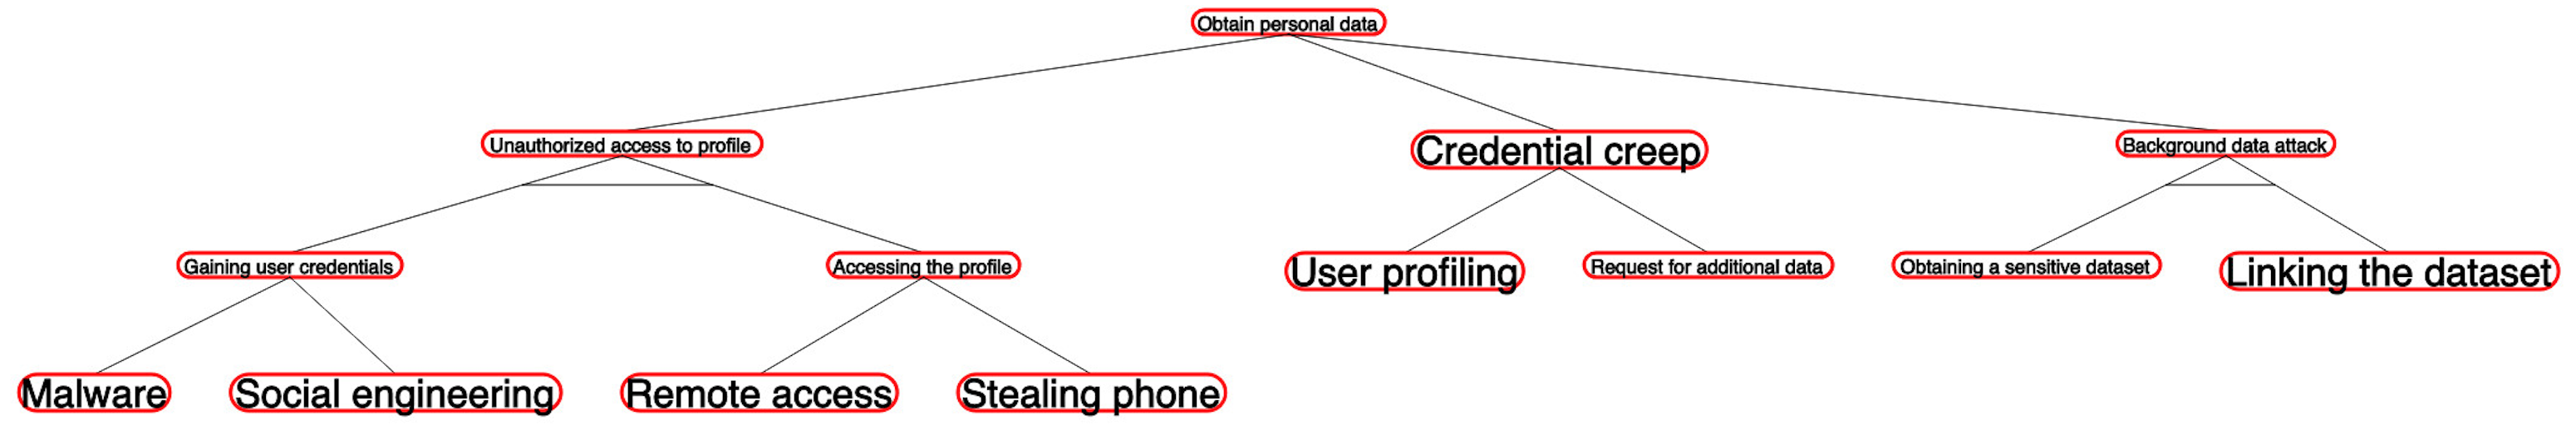
\includegraphics[width=\linewidth]{img/TargetAT.png}
%     \caption{An attack tree adapted from Naik \etal~\cite{naikEvaluationPotentialAttack2022} that is used in the study described in Section~\ref{sec:methodology}. }
%     \label{fig:tartgetAT}
% \end{figure*}



\begin{figure*}
\resizebox{\linewidth}{!}{
    \begin{forest}
        for tree={
        draw,
        minimum height=.25cm,
        anchor=parent,
        align=center,
        child anchor=parent,
        edge=-
        },
        adnode/.style={rounded rectangle,},
        [{Obtain personal data}, adnode,
                [{Unauthorized access to profile}, adnode, small angle below,  [{Gaining user credentials}, adnode,[{Malware}, adnode,][{Social engineering}, adnode,]] [{Accessing the profile}, adnode,[{Remote access}, adnode,][{Stealing phone}, adnode,]]]
                    [{Credential creep}, adnode,  [{User profiling}, adnode,] [{Request for additional data}, adnode,]]
                    [{Background data attack}, adnode, small angle below, [{Obtaining a sensitive dataset}, adnode,] [{Linking the dataset}, adnode,]]
            ]
    \end{forest}
}
\caption{An attack tree adapted from Naik~\etal~\cite{naikEvaluationPotentialAttack2022} that is used in the study described in Section~\ref{sec:methodology}. }
    \label{fig:tartgetAT}
\end{figure*}

% \begin{figure*}
%     \resizebox{\linewidth}{!}{
%         \begin{forest}
%             for tree={
%             draw,
%             minimum height=.25cm,
%             anchor=parent,
%             align=center,
%             child anchor=parent,
%             edge=-
%             },
%             adnode/.style={rounded rectangle,},
%             [{Obtain personal data}, adnode,
%                     [{Unauthorized profile access}, adnode, small angle below,
%                             [{Gaining user cred.}, adnode,
%                                     [{Malware}, adnode,]
%                                         [{Social engineering}, adnode,]]
%                                 [{Access profile}, adnode,
%                                     [{Remote access}, adnode,]
%                                         [{Steal phone}, adnode,]]]
%                         [{Background data attack}, adnode, small angle below,
%                             [{Obtain dataset}, adnode,]
%                                 [{Link dataset}, adnode,]]
%                         [{Cred. creep}, adnode,
%                             [{User profiling}, adnode,]
%                                 [{Request additional data}, adnode,]]
%                 ]
%         \end{forest}
%     }
%     \caption{An attack tree that was also adapted from Naik~\etal~\cite{naikEvaluationPotentialAttack2022} which should be equivalent to Figure~\ref{fig:tartgetAT}. This will be used in Section~\ref{sec:distance} to model the different distance measurements.}
%     \label{fig:tartgetAT2}
% \end{figure*}

We define attack trees, as initially described by Bruce Schneier~\cite{schneierAttackTrees1999}, to be a rooted acyclic structure with the following recursive definition  from Gadyatskaya~\etal~\cite{gadyatskayaRefinementAwareGenerationAttack2017}.

\begin{definition} \label{def:attack-tree}

An attack tree $t$ is defined as:
\[
    t = b | b\Delta(t_1, ..., t_i)
\]

Where $b \in \mathbb{B}$ is an action or goal in service of an attack, where $\mathbb{B}$ is the set of all possible attack components. For our purposes, $b$ is considered the label of a node. $\Delta$ is the refinement of a node, giving the relationship between child nodes. For our purposes, $\Delta$ is either \AND\ or \OR.



% An attack tree  is defined as $T = \ATnode{1}{1}\Delta(\ATnode{2}{1},...,\ATnode{2}{i})$. Where $\ATnode{d}{i} = \ATlabel{d}{i}\Delta(\ATnode{d+1}{j},...,\ATnode{d+1}{k})$

    % We define the $i\text{th}$ node according to left-right post-order number to be the following, $T[i] = b\Delta(T[j],...,T[k])$. 

    % We give $b$ to be some action within the attack scenario, which is the node label of $t$. For clarity, we additionally refer to this label as $t.\text{label}$. We give $\Delta$ to be the refinement $\Delta = \AND|\OR|\SAND$. For clarity and consistency, we refer to the refinement of a given node to be $t.\Delta$. Following the refinement, we have a list of nodes which are the children of $t$, defined as $t_0,...,t_i$ which is the left to right order of the children (regardless of if order is significant). We refer to the list of children as $t.\text{children}$. This list of nodes can be empty, in the case of leaf nodes.

    % For clarity and consistency, we refer to the refinement of a given node to be $t.\Delta$. Following the refinement, we have a list of nodes which are the children of $\ATnode{d}{i}$, defined as $\ATnode{d+1}{j},...,\ATnode{d+1}{k}$ where $j \ge 1$ and $k \ge j$, which is the left to right order of the children (regardless of if order is significant). We refer to the list of children as $\ATnode{d}{i}.\text{children}$. This list of nodes can be empty, in the case of leaf nodes.

% Each node within an attack tree is a sub-tree unto itself. We define each node as $\ATnode{d}{i}$ where $d$ is the depth of the node (distance from the root, given the root has a starting distance of 1), and $i$ is the number of that node counting from the left most node at depth $d$ (starting from 1). We define a mapping of each node to a label space, where the label of node $\ATnode{d}{i}$ is given as $\ATlabel{d}{i}$. We give $\Delta$ to be the refinement $\Delta = \AND|\OR$. We further define the following functions to retrieve associated information of some node $\ATnode{d+1}{j}$. We define the $\Delta(\ATnode{d}{i})$ function to return the refinement of a given node. We define the child function, $\childFunc{\ATnode{d}{i}}$ to return a list of nodes which are the children of a given node, defined as $\ATnode{d+1}{j},...,\ATnode{d+1}{k}$ where $j \ge 1$ and $k \ge j$, which is the left to right order of the children (regardless of if order is significant). This list of nodes can be empty, in the case of leaf nodes. Finally, we define the parent function, $\parentFunc{\ATnode{d}{i}}$ to return the parent of a given node.
\end{definition}

Fundamentally, distance measures provide a means of comparison, and means of comparison are critical for any industry. New applications of distance measures are easily found once the distance measure to defined~\cite{beham2011new}. We propose two potential uses of these distance measures; however, future work will further specify new applications. Threat models are a recommended tool for threat analysis~\cite{andersonSecurityEngineeringGuide2020,schneierSecretsLiesDigital2000}. However, once these models are created, they may only be applicable to the analyst or the team of analysts that created them. Unlike other sources of threat intelligence, such as YARA Rules~\cite{naik2019cyberthreat,naik2020evaluating}, there is no means to share attack trees in this format.

In order to allow for attack trees to be shared as threat intelligence, two aspects are needed: a common structure and a means of comparison. The common structure has already been defined, in the ADTool XML Schema~\cite{kordy_adtool_2013}. This is an XML format used by ADTool, a tool to create Attack-Defense Trees, an extension of ATs. The ADTool XML Schema can be used to define attack trees, and as such, can be used as a common structure for sharing attack trees. The dataset of ATs we describe in Section~\ref{sec:results} is in this format. The second aspect is a means of comparison, which is what we have defined in this paper. It will be possible to publish attack trees in the ADTool XML Schema, and then compare the resulting trees using the distance measures we have defined. This will allow for the sharing of attack trees as threat intelligence, and the comparison of these trees to identify similar threats.

% \subsubsection{Generative AI}

% Applying generative AI to security is an active area of research. Distance measures are critical for using generative AI to create threat models in general, and attack trees specifically. By using a distance measure, we can compare the output of a generative AI to a set of known attack trees, and determine how similar the output is to the known attack trees. As we can control the form of the output of generative AI, we can have an AI tool output AT in the ADTool XML Schema, and then compare the resulting attacks to our own output or to a dataset.

% Going further, in order to build and refine a generative AI tool to create attack trees, most method will require a cost function to be defined~\cite{bottou1991stochastic}. A cost function is necessary for most model training, as this is what the model will attempt to optimize for. Fundamental to this cost function is the ability to define distance, as we can offer a way to compare a generated solution to a ``ground truth''. Beyond this, distance measures can be used to better define which and how artificial intelligence systems should be applied to attack trees, as was shown by Terry Jones~\cite{jones1995fitness}.


%\section{Research}

% Our primary research goal is to determine a mechanism to calculate the distance between two attack trees. This is a novel problem, as attack trees contain the concept of refinements, and the application of tree edit distance to the cybersecurity domain has yet to be seen.


\section{Requirements}
\label{ssec:requirements}

We have defined a number of requirements to compare attack trees. These requirements are subsequently used in Section~\ref{sec:methodology} to inform our study design.

\subsection{Theoretical Requirement}

Our main theoretical requirement is that the distance between two attack trees must be a \textbf{metric}. That is to say, the distance between two attack trees must be non-negative, symmetric, and satisfy the triangle inequality. This is a fundamental requirement for any distance measure, as it ensures that the distance between two trees is a meaningful value. Futher, the distance measure should incorporate all aspects of a tree, including \textbf{position} of nodes within the tree, the \textbf{refinement} of nodes, and the \textbf{labels} of nodes. Finally, our distance measure should work on \textbf{unordered} attack trees, as the standard definition of attack trees does not assign an order to children of nodes~\cite{mauw_foundations_2006}.


\subsection{Usability Requirements}

As we are motivated by a desire to produce a metric has applications for practitioners, we have a number of requirements we expect a potential distance measure to meet. These requirements are as follows:
We expect our distance measure to be able to describe distance between trees with \textbf{unfiltered} labels. A practitioner should be able to apply this distance measure without needing compared trees to have identical node labels; human developed labels can be noisy, and our distance measure should have some mechanism to compare these labels meaningfully. We expect that the distance measure we find is \textbf{intuitive}ly understandable by a user; in other terms, a practitioner should be able to easily roughly understand why two trees are a given distance apart.





% \subsubsection{Validation Requirements}

% We must be able to validate these measures, which we will be able to do if the trees respond in a predictable manner and intuitive manner. 












% 



\subsection{Other considerations}

Most attack trees are drawn for specific situation by individual practitioners, with the largest trees being in the 100s of nodes; we would consider an exceptionally large tree to be on the order of magnitude of 1000 nodes. As such, it should be unnecessary to optimize for complexity, as attack trees, especially human drawn attack trees, do not reach the size where complexity becomes a significant issue. Even in the case of a large dataset of attack trees, due to the relatively small size of each individual attach tree, the complexity of a distance calculation should not impact computability. Therefore, we so not consider computational complexity as a requirement for our distance measurement.

We are examining the distance between trees that are correctly formed. We do not define potential distance values for trees that have some form of structural error. We assume that the compared attack trees follow all defined composition rules~\cite{mauw_foundations_2006}. Further, for the ``unfiltered'' trees we examine in Section~\ref{sec:results}, all trees are defined according to the ADTool XML Schema, which functionally guarantees that all tree are well formed~\cite{kordy_adtool_2013}.


















% The application of tree edit distance to attack trees requires a number of considerations. These considerations are as follows:

% \subsubsection{Simple definition of difference}

% We aim to establish some means by which we can say that some tree $T_A$ differs from some tree $T_B$ by some amount $x$. This description of difference should be simple and intuitive, such that a practitioner can understand the difference between two trees without needing to understand the underlying mathematics.

% \subsubsection{Applicable to unfiltered trees}

% As the ultimate goal is to find a mechanism that is usable for attack trees that are drawn by practitioners. As such, the distance calculation must be effective and meaningful to trees that are not filtered or otherwise processed. 

% \subsubsection{Effect size}

% This distance between two attack trees should be indicative of how different the two trees. 


% \subsubsection{Detailed description of difference}

% The calculation of a distance must produce a description of the difference between two trees. This description should be human readable and should be able to be used to inform a practitioner of the differences between two trees.

% \subsubsection{Can handle unordered trees}

% The distance calculation must incorporate all elements of attack trees. This includes the refinement  and the labels of nodes, for all nodes in the tree.

% \subsubsection{Incorporates all elements of attack trees}

% The distance calculation must incorporate all elements of attack trees. This includes the refinement, position,  and the labels of nodes, for all nodes in the tree.

% \subsubsection{Difference is a metric}

% The distance between two attack trees must be a metric. That is to say, the distance between two attack trees must be non-negative, symmetric, and satisfy the triangle inequality.



% \subsection{Assumptions}

% We make a series of assumptions in our comparisons of attack trees. These assumptions are as follows:  

% \subsubsection{Attack tree size}

% We assume that attack trees are of a relatively small size. In a previous study on self drawn attack defense trees, the largest attack trees were on the order of 50 nodes. While this is large for a human to comprehend, on the scale of data structures, this is miniscule. As such, it should be unnecessary to optimize for complexity, as attack trees, especially human drawn attack trees, do not reach the size where complexity becomes a significant issue. Even in the case of a large dataset of attack trees, due to the relatively small size of each individual attach tree, the complexity of a distance calculation should not impact computability. Therefore, we so not consider computational complexity as a requirement for our distance measurement.

% \subsubsection{Attack trees are correctly formed}

% We are examining the distance between trees that are correctly formed. We do not define potential distance values for trees that have some form of structural error. We assume that the compared attack trees follow all defined composition rules~\cite{mauw_foundations_2006}. Further, for the ``unfiltered'' trees we examine in Section~\ref{sec:results}, all trees are defined according to the ADTool XML Schema, which functionally guarantees that all tree are well formed~\cite{kordy_adtool_2013}.


% \subsubsection{Refinement Awareness}
% \label{sssec:refinement}

% The primary difference between attack trees and most directed acyclic graphs (DAGs) are the presence of refinements, or the given relationship between children. This is a critical part of the attack tree structure and must be included in the tree edit distance algorithm.

% \subsubsection{Semantic Label Similarity}
% \label{sssec:label-similarity}

% In early iterations of tree edit distance problems, node labels were said to be equivalent if the labels were identical. However, in most contexts, it will not be the case that node labels will be identical. Especially in the context of cyber security, it is easily possible for two nodes in a DAG to represent the same idea but presented in a radically different manner. As such, the distance between attack trees must have a mechanism to account for the similarity between node labels on the basis of their meaning.

% \subsubsection{Order of children}
% \label{sssec:order-of-children}

% It is a known problem that tree edit distance of unordered trees is an \textit{NP}-Complete problem~\cite{zhang_editing_1992}. However, attack trees are unique in that the order of children is dependent on the refinement of the parent node. As such, the distance between attack trees must be able to account for the order of children in the context of the refinement of the parent node. In the case of \AND\ and \OR\ refinements, the children are unordered. However, in the case of \SAND\ (\emph{Sequential} \AND) refinements, the order of children is important. As such, the edit distance between two attack trees must optimize to allow for the reordering of nodes when calculating the edit distance; however, this optimization must be such that it is selectively applicable, and can be not applied in the case of \SAND\ refinements.

% \subsubsection{Metric}
% \label{sssec:metric}

% The distance between two attack trees must be a metric. That is to say, the distance between two attack trees must be non-negative, symmetric, and satisfy the triangle inequality.



% \subsubsection{Consensus Trees}
% \label{sssec:consensus-trees}

% \NS{I dunno if this should be included in this paper - but it'd make it SO MUCH EASIER to argue utility}


% One potential utility of tree edit distance would be to allow for the recognition missing vectors or components of attack trees \NS{cite AG distance paper}. For example, if we find that one tree is a whole subset of another tree, that is the consensus tree between two trees is equivalent to one of the trees, then we can infer that the components of the larger tree are components that would be directly applicable to the subset tree. As such, we can use this method of calculating a consensus tree to find missing components of attack trees.





\section{Related Work}
\label{sec:related-work}

Distance between data structures is not a new concept. Many works have explored the idea of ``distance'' between strings. In string edit distance, where the difference in strings is given my a min-cost path taken by either adding a character, removing a character or replacing a character. By fining the minimum cost needed to transform one string into another, a ``distance'' value can be given. The cost of transformation increases with the difference between two strings~\cite{yujianNormalizedLevenshteinDistance2007, masekFasterAlgorithmComputing1980}.

Tree edit distance is seen as an extension of the string edit distance problem. Tai first tackled the problem, suggesting an edit distance metric for two directed acyclic graphs (DAG)s \cite{tai_tree--tree_1979}. Zhang and Shasha have written the seminal work on tree edit distance~\cite{zhang_simple_1989}. In their work, they describe a simple algorithm for calculating the distance between two trees. This algorithm is based on the idea of a \textit{forest} distance, which is the distance between two forests. A forest is possible disjoint a collection of trees, though a forest can consist of a single tree. The distance between two forests is the minimum cost of transforming one forest into another. This is calculated by finding the minimum cost of transforming each tree in the first forest into each tree in the second forest. This is done recursively until the minimum cost of transforming each node in the first tree into each node in the second tree is found. The minimum cost of transforming the first tree into the second tree is then given as the optimal \emph{tree edit distance} between two trees. This edit distance is given as both a value, the cost of the sequence of edits, as well as the sequence of edits itself. This sequence of edits has 3 possible operations.

Most of the research and development on tree edit distance focuses calculation optimization. As shown by Zhang~\etal, the tree edit distance problem for unordered trees is an \textit{NP}-Complete problem~\cite{zhang_editing_1992}. As such, the development of novel optimal calculation strategies is necessary to enable comparison of larger tree structures. Yoshino \etal\ developed a dynamic programming A$^*$ algorithm for computing unordered tree edit distance (UTED), which offer significant performance gains over exhaustive search~\cite{yoshino_dynamic_2013}. Their method uses an A$^*$ algorithm to construct a search tree of mappings. The distance is then calculated from these mappings. Unfortunately, these mapping rely on an absolute equivalence between nodes to establish a mapping, which will not exist in ``unfiltered'' attack trees, and thus cannot be applied in our case. However, the intuition to optimize finding mappings and then find the distance based on the mappings is a useful methodology that we can apply to our work. Other work based on the A$^*$ algorithm methodology, such as the optimizations offered by Paaßen~\cite{paasen_-algorithm_2021} for computing UTED will have the same unsuitability.

McVicar~\etal\ have developed a method of calculating UTED in SuMoTED by focusing on allowing nodes to move up or down a tree and organizing edits around a consensus tree~\cite{mcvicar_sumoted_2016}. This methodology allows them to achieved polynomial time calculation of UTED. However, application of this methodology to attack trees presents difficult. Namely, the same issue as the A$^*$ algorithm, the requirement of exact equivalence between node labels.

% McVicar~\etal\ have developed a method of calculating UTED in SuMoTED by focusing on allowing nodes to move up or down a tree and organizing edits around a consensus tree~\cite{mcvicar_sumoted_2016}. This methodology allows them to achieved polynomial time calculation of UTED. However, application of this methodology to attack trees presents difficult. Namely, the same disallowance of ordered nodes. Additionally, by allowing movement of nodes below leaf nodes would functionally introduce a refinement to the attack tree, which would require a new mechanism to accomodate this potential action. In effect, unlike SuMoTED, movement of nodes up a tree would not be equivalent to movement of nodes down a tree, and this equivalence is assumed in SuMoTED.

Pawlick and Augusten proposed RTED, a more optimal method of calculating ordered TED (OTED)~\cite{pawlik_rted_2011}. Their methodology is faster than Zhang and Shasha, but specifically for larger trees (500+ nodes). Attack trees by contrast cannot grow this large as they become unable as threat models~\cite{andersonSecurityEngineeringGuide2020}. As such, RTED, while an important optimization and contribution, does not offer a significant advantage for attack trees over Zhang and Shasha.

% Tree edit distance, like string edit distance, has a wide array of applications. Just as string edit distance has been used to compare sequences of DNA \NS{ cite},






% Much of the work in this field has built upon work by Kuo-Chung Tai who suggested that the distance between trees is similar to several previous works comparing the differences in strings~\cite{tai_tree--tree_nodate}.


% In the Zhang and Shasha algorithm the three possibilities for an edit operation between individual nodes are, (i) a node must be added, (ii) a node must be removed, or (iii) a node must be replaced~\cite{zhang_simple_1989}. Each of these operations has a cost

% Zhang and Shasha proposed a commonly cited simple algorithm for calculating tree edit distance~\cite{zhang_simple_1989}. We use this algorithm in this paper as it is a common strategy for implementing and testing extensions to tree edit distance. As such, optimizations based on the Zhang and Shasha algorithm can be applied to our methodology as we show in section \NS{When I write that section, I'll reference it here}.
\section{Validation}
\label{sec:validation}

In order to evaluate any approach for comparing attack trees, we must first establish a means of validating the results and assessing the quality of this approach. We propose two methods of validating the distance measures:

\textbf{Theoretical validation}. This validation method involves defining a series of basic transformation examples (BTEs) that represent the most fundamental ways in which two attack trees could differ from each other. These BTEs can be adapted to only express the transformations that we would expect to see, or that we explicitly would desire to compare two distance measures along. For example, if we only wish to evaluate distance measures according to their ability to compare leaf nodes (as the traditional attack tree semantics expect~\cite{mauwFoundationsAttackTrees2006}), we could define a set of BTEs which only shows changes in leaf nodes. For a more comprehensive comparison, we can define a larger set of BTEs to show all possible basic transformations. This is what we do in Section~\ref{sec:methodology}. We argue that if any transformation can be expressed as a series of BTEs, then we can validate the distance measure by comparing the distance measure's output to the expected distance of each BTE.

\textbf{Experimental validation}. We offer an experimental design that can be used to validate a distance measure on ``real-world'', human-produced data. This requires a dataset that contains two sets of attack tree models. First, we require a base set of trees which should all be identical. This can be created by asking participants to create an attack tree describing the same precisely defined scneario. Any variation between the trees would likewise be representative of ``real-world'' label variation, and not due to differences in attack steps identified by distinct experts. In this way, we can evaluate how the distance measures handle similar but not fully identical data. 

Second, we require the base set of trees to be slightly expanded by the authors. This results in a second set of trees that are expected to be slightly different, but not very diverse. At the same time, the base set contains attack trees that are subtrees of this second set. This allows us to evaluate the behavior of the distance measures when comparing a tree to a known subset of that tree, and to compare a set of attack trees that are slightly different from each other. This behavior should be predictable, and we can access distance measures if they display the behavior we expect. We describe the details of our study design and the data collection process in Section~\ref{sec:methodology}.
\section{Semantic Similarity}
\label{sec:semantic-similarity}


\tikzstyle{block} = [rectangle, draw, fill=black!290,
text width=5em, text=white,  text centered, rounded corners, minimum height=4em]
\begin{figure*}
    \centering
    \begin{tikzpicture}[node distance = 2cm, auto]
        % Place nodes
        \node [xshift=-5cm](t1) {$\ATlabel{d}{i}$};
        \node [below of = t1] (t2) {$\ATlabel{e}{j}$};
        \node [block, below right = .5cm and 1cm of t1, yshift=.3cm]  (genbeddings) {\shortstack{Generate\\Semantic\\Embeddings}};
        \node [right of = t1, xshift=4cm]  (et1) {$\vec{e}(\ATlabel{d}{i})$};
        \node [below of = et1]  (et2) {$\vec{e}(\ATlabel{e}{j})$};
        \node [block, right of = genbeddings, xshift= 4.5cm]  (comp) {\shortstack{Vector\\Comparison}};
        \node [right of = comp, xshift = 2cm]  (end) {$\delta(\ATlabel{d}{i}, \ATlabel{e}{j})$};


        % Draw edges
        \draw [->] (t1.east)  -| ($(t1)!0.5!(genbeddings)$) coordinate |-(genbeddings);
        \draw [->] (t2.east)  -| ($(t2)!0.5!(genbeddings)$) coordinate |-(genbeddings);
        \draw [->] (genbeddings.east)  -| ($(genbeddings)!0.5!(et1)$) coordinate |-(et1);
        \draw [->] (genbeddings.east)  -| ($(genbeddings)!0.5!(et2)$) coordinate |-(et2);
        \draw [->] (et1.east)  -| ($(et1)!0.5!(comp)$) coordinate |-(comp);
        \draw [->] (et2.east)  -| ($(et2)!0.5!(comp)$) coordinate |-(comp);
        \draw [->] (comp)  -- (end);
    \end{tikzpicture}
    \caption{Process of calculating the distance between two node labels.}
    \label{fig:semanticreplacement}
\end{figure*}

In most of the tree distance measures described in Section~\ref{sec:related-work}, nodes are only matched, or considered equivalent, if the node labels are identical. Taking one example from our experiment (described in Sections~\ref{sec:methodology}~and~\ref{sec:results}), this would result in the node labels ``Obtain personal data'' and ``obtain personal data'' to not be matched, as these labels are not identical. While other label reconciliation schemes have been proposed, many are based on the string edit distance (Levenshtein distance) of the two node labels. This method is not ideal as it can result in two nodes that are entirely unrelated but with similar vocabulary having small edit distances, while two nodes that are related or identical having large edit distances. In Table~\ref{tab:distances}, we provide a few examples of potential node label comparisons using both normalized Levenshtein distance and semantic similarity. Semantic similarity is calculated using the BERT method and is shown graphically in Figure~\ref{fig:semanticreplacement}. The normalized Levenshtein distance is calculated as one minus the Levenshtein distance divided by the length of the longest string:

\[
\delta\left(\ATlabel{d}{i}, \ATlabel{e}{j}\right) = 1 - \frac{\text{Levenshtein}\left(\ATlabel{d}{i}, \ATlabel{e}{j}\right)}{\max\left(\left|\ATlabel{d}{i}\right|, \left|\ATlabel{e}{j}\right|\right)}
\]

% \[
% \delta(b_i, b_j) = 1 - \frac{\text{Levenshtein}(b_i, b_j)}{\max(|b_i|, |b_j|) }
% \]


In Table~\ref{tab:distances}, can see the extreme example of ``door open'' and ``open door'' which has a Levenshtein distance of 8 (normalized Levenshtein distance of 0), as all letters must be changed. However, the semantic similarity is 0.992, which is the highest of our selected examples. This is because the two labels are near identical in meaning, and the only difference is the order of the words. In contrast, the two labels ``obtain personal data'' and ``obtain personnel'' have a normalized Levenshtein distance of .5882, but a semantic similarity of 0.4507. This is because the two labels are not related, but due to similar language, the normalized string edit distance is relatively small. If we implemented a distance between the two labels
$\delta\left(\ATlabel{d}{i}, \ATlabel{e}{j}\right)$ %$\delta\left(\ATlabel{d}{i}, \ATlabel{e}{j}\right)$ 
to be based on Levenshtein distance, nodes that should be considered equiavelnt to be different and nodes that should be considered different to be equivalent.
% This method is not ideal, as it is possible for two unrelated nodes to have small edit distances, such as ``obtain personnel'' and ``obtain personal data'' (edit distance of 7) while related nodes have larger edit distances; such as comparing ``obtain personal data'' and ``gather private info'' (edit distance of 15). In our first example, the two nodes are not related, but due to similar verbiage, the edit distance is relatively small. In the second example, the two nodes have identical meaning, but due to different vocabulary used, the Levenshtein distance between them is significantly larger. If we implemented a distance between the two labels  $\delta\left(\ATlabel{d}{i}, \ATlabel{e}{j}\right)$ to be based on Levenshtein distance, nodes that should incur a cost to edit may not while those that should not incur a cost to edit may.

\begin{table}[]
    \begin{tabular}{@{}llll@{}}
        \toprule
        Label 1              & Label 2             & \begin{tabular}[c]{@{}l@{}}Normalized\\Levenshtein\\ Distance\end{tabular} & \begin{tabular}[c]{@{}l@{}}Semantic \\ Similarity\end{tabular} \\ \midrule
        obtain personal data & obtain personnel    & 0.5882                                                                     & 0.4507                                                         \\
        obtain personal data & gather private info & 0.1176                                                                     & 0.5521                                                         \\
        break open safe      & break open door     & 0.6923                                                                     & 0.7855                                                         \\
        break open safe      & crack safe open     & 0.1538                                                                     & 0.814                                                          \\
        crack safe           & crack door          & 0.5556                                                                     & 0.6692                                                         \\
        door open            & open door           & 0.0                                                                        & 0.992                                                          \\ \bottomrule
    \end{tabular}
\caption{Select examples of potential node label comparisons using both Levenshtein distance and semantic similarity. Semantic similarity is calculated using the methodology shown in Figure~\ref{fig:semanticreplacement}.}
    \label{tab:distances}
\end{table}



What we subsequently would desire is a method of comparing the two labels and making a determination of whether or not nodes are the same based on meaning. If nodes have identical, or relatively identical, meanings, then the cost of replacement should be 0 (\textit{i.e.} matching). If the nodes have dissimilar meanings, then the cost of replacement should be greater than $0$. We can achieve this by generating semantic embeddings for each node label, and comparing the resulting embeddings. If the semantic similarity is above a given threshold, $\epsilon$, we give the cost of replacement to be 0; otherwise, we give the cost of replacement to be 1. This allows for the Zhang and Shasha algorithm to replace nodes with similar labels at a lower cost than nodes with dissimilar labels.


\subsection{Threshold Problem}
\label{sssec:threshold-problem}

Equivalence is a binary measurement, either labels are equivalent or not. In order to ensure comparability of distance measures, all of the distance measures proposed in the Section~\ref{sec:distance} require a binary determinations of matching (equivalent) or changing (not equivalent). While it may be the case that allowing more nuanced determinations of similarity make result in more nuanced tree distance measures, this would limit our ability to compare the distance measures. By simplifying the distance measures along this metric, we increase our ability to compare the distance measures based on behavior.

However, semantic similarity is a continuous value between 0 and 1, which by its nature is not binary. In order to convert this continuous measure of semantic similarity to one of semantic equivalence, we employ a threshold value of $\epsilon$. Any semantic similarity value above $\epsilon$ is considered equivalent, and any semantic similarity value below $\epsilon$ is considered not equivalent.

Thus, we encounter the threshold problem; the problem of defining a threshold $\epsilon$ for the semantic similarity between two labels. This threshold is necessary to determine if two labels are similar enough to be considered the same. We do not offer a mechanism to account for partial similarity. This could be allowed, but would present a similar problem to the threshold problem; namely, where to set $\epsilon$. We simplify our calculation by not allowing partial calculations, and in Sections~\ref{sec:results}~and~\ref{sec:discussion}, we examine the effect of different $\epsilon$ on the results of our distance calculation.

\section{Distance Measures}
\label{sec:distance}

In this section, we describe the distance measures that we use to compare attack trees. 


\begin{figure*}
    \centering
    \begin{subfigure}[b]{.40\linewidth}
        \resizebox{\linewidth}{!}{
            \begin{forest}
                for tree={
                draw,
                minimum height=.25cm,
                anchor=parent,
                align=center,
                child anchor=parent,
                edge=-
                },
                adnode/.style={rounded rectangle,},
                [{Gain Access}, adnode,
                        [{Find unlocked computer}, adnode,]
                            [{Phishing}, adnode, small angle below
                                    [{Send Email}, adnode,]
                                    [{Receive Credentials}, adnode,]]
                    ]
            \end{forest}
        }
        \caption{A simple attack tree.}
        \label{fig:dist-example-1}
    \end{subfigure}
    \begin{subfigure}[b]{.57\linewidth}
        \resizebox{\linewidth}{!}{
            \begin{forest}
                for tree={
                draw,
                minimum height=.25cm,
                anchor=parent,
                align=center,
                child anchor=parent,
                edge=-
                },
                adnode/.style={rounded rectangle,},
                [{Gain Unauthorized Access}, adnode,
                        [{Phishing}, adnode, small angle below
                                    [{Send Phishing Email}, adnode,]
                                    [{Get Credentials}, adnode,]]
                            [{Find open computer}, adnode,]
                            [{Brute force}, adnode,]
                    ]
            \end{forest}
        }
        \caption{A slightly modified attack tree.}
        \label{fig:dist-example-2}
    \end{subfigure}
    \caption{Two similar attack trees with small differences to model the distance measures.}
    \label{fig:dist-example}
\end{figure*}

% \subsection{Measurement Comparison}

% A comparison of a series of measurements of two attack trees. These measurements could include, but would not be limited to, the number of nodes, the number of leaf nodes, the number of refinements, the number of \AND\ and \OR\ refinements, the depth of the tree, and the average number of children per node. By comparing this series of measurements, we can roughly describe the difference between two attack trees. This means of measuring the difference between two trees has been used in lieu of a more established difference mechanism.

% \NS{I'm refering to myself in acceptability 1}

\subsection{Label Distance}
\label{ssec:label-distance}

Label Distance (LD) is a measure of the difference between the labels of a given tree. This is derived from the mappings suggested in Tai~\cite{tai_tree--tree_1979} and Zhang and Shasha~\cite{Zhang_Shasha_1989}, with an algorithm influenced by the A$^*$ tree edit distance algorithm from Yoshino~\etal~\cite{yoshino_dynamic_2013}. We can calculate the distance between two labels by using a pre-trained BERT model to calculate the semantic similarity between two labels. This is done by calculating the cosine similarity between the embeddings of the two labels. This is shown in Figure~\ref{fig:semanticreplacement}. We create a matrix $D$ which is an $M \times N$ matrix which represents all of the distances between the labels between two trees. We then take the largest value at index $i, j$ of this matrix and remove that row ($i$) and column ($j$) from $D$, recording the mapping between $b_i$ and $b_j$. This is repeated until all nodes are included in a mapping set. If the largest value in $D$ is below some value $\epsilon$, we consider the labels to be different, and a direct mapping is not created. We add the nodes as individuals to the mapping (mapping to/from $\Lambda$ indicating that these labels would be removed or added). We then calculate the cost of each node that would be removed or added, giving a cost of 1. This algorithm is defined in detail in Algorithm~\ref{alg:label-distance} in Appendix~\ref{appendix:alg:label-distance}. We can divide this value by the number of nodes in the largest tree to get a normalized value.



This measurement considers all the labels of each node within an attack tree. It uses a semantic comparison to examine the meanings of the nodes, which would allow for this distance measure to work on unfiltered trees. However, this measure does not consider the structure of the tree in any way, and therefore does not represent how the nodes are organized. If we examine the attack tree in Figure~\ref{fig:tartgetAT}, if create an attack tree with all the same label names, but all nodes directly attached to the root (a single root node with 13 child nodes with identical names as in Figure~\ref{fig:tartgetAT}), the resulting label distance would be zero. As such, label distance offers a way to quickly examine if the meanings of the nodes are similar, but does not offer a way to examine the structure of the tree. 

Label distance is functionally a Jaccard distance on two sets of labels. As Jaccard distance follows the triangle inequality~\cite{kosub2019note}, it follows that LD follows the triangle inequality. As LD is additive, it cannot be negative; further, the distance between identical sets is 0. Therefore, LD is a metric.


Applying LD to the examples provided in Figure~\ref{fig:dist-example}, we would first create two lists of labels of both Figures~\ref{fig:dist-example-1}~and~\ref{fig:dist-example-2}. Then we could compare these lists according to their semantic similarity along the process described in Section~\ref{sec:semantic-similarity}. The labels that are identical will be matched first, then the labels will be matched according to their semantic similarity in decreasing order. This is repeated until only the node ``brute force'' from Figure~\ref{fig:dist-example-2} remains. Provided all other nodes match (given a sufficiently permissive value of $\epsilon$), LD will result in a distance of 1 (normalized distance of 0.167).



\subsection{Tree Edit Distance}
\label{ssec:ted}

Tree edit distance is a measure of the difference between two trees by defining an optimal edit path; that is, what changes are needed to turn one tree into another. The seminal work in this field is by Zhang and Shasha~\cite{Zhang_Shasha_1989}. In their work, they describe a simple algorithm for calculating the distance between two trees. This algorithm is based on the idea of a \textit{forest} distance, which is the distance between two forests, or sets of trees. The result of this algorithm is a measure of the costs of edits needed to transform one tree into another, with the convention being that any edit requires a cost of 1. The possible edits are matching, in which two nodes are defined to be equivalent which is the only edit without cost. Insertion in which a node is added, deletion in which a node is removed, and changing one node into another, in which a node has its label replaced. We modify the Zhang and Shasha algorithm in three ways, we introduce a mechanism for comparing the semantic meaning of node labels (similar to label distance) and a new cost for changing the refinement of a node. It is possible to take this absolute edit distance number and divide it by the tree with the largest number of nodes to find a normalized value. Li and Chenguang proved that the non-normalized TED is a metric~\cite{li2011metric}.

The tree edit distance from Zhang and Shasha works on ordered trees, which for our purposes presents a challenge, as our attack trees are unordered. Zhang~\etal showed that unordered tree edit distance is a MAX SNP-Hard problem~\cite{zhang_max_1994}. Our assumption that attack trees do not grow to be very large allows us to remain unconcerned about the processing time of unordered tree distance. Previous work on unordered tree edit distance has offered various polynomial time approximate solutions, all making assumptions to speed up computations. Fundamentally, all make the same assumption, which is that there is absolute equivalence between nodes within two trees. Either nodes have identical labels or they do not. This would preclude their use on unfiltered data, as nodes are not guaranteed to have the same label. On unfiltered data, these algorithms may find a local maximum instead of the global maximum needed to create a mapping (as is done in label distance described in Section~\ref{ssec:label-distance}) has an issue of assuming nodes with absolute equivalence. That is, each algorithm will assume a mapping that may not be optimal if it finds two nodes to be ``equivalent'' if their similarity is above a given threshold (see Section~\ref{sssec:threshold-problem}), or it will not find a mapping between most similar nodes because these nodes do not have identical labels. As such, these algorithms are unsuitable for our purposes.


Applying TED to the examples provided in Figure~\ref{fig:dist-example}, we follow the process described in \cite{Zhang_Shasha_1989}, by calculating key roots (the rightmost parent of each subtree) and then computing forest distance. For the specific mechanics of this distance, we refer the reader to the work by Zhang and Shasha~\cite{Zhang_Shasha_1989}. The resulting distance given a reasonable value of $\epsilon$ is 5 (normalized to 0.833). This is higher than for the other distance metrics as this implementation of TED is unable to handle reordered nodes.
Figures~\ref{fig:dist-example-1}~and~\ref{fig:dist-example-2}


% \subsubsection{Refinement Cost}
% One of the biggest differences between attack trees and other tree-like data structures is the presence of refinements, or the \AND\ and \OR\ relationships, which state whether all of the children of a node must be satisfied for the parent node to be satisfiable (\AND) or if at least one must be satisfied for a parent node to be satisfiable (\OR). This is a critical part of the attack tree structure and must be included in the tree edit distance algorithm.




% \begin{definition}\label{def:cost-function}
%     Similar to Zhang and Shasha, we define $\gamma$ be the cost function for the node edit distance, with the cost of removing a node to be $\gamma(\ATnode{d}{i} \rightarrow {\Lambda})$, the cost of adding a node to be $\gamma({\Lambda}\rightarrow \ATnode{d}{i})$, and the cost of changing a node to be $\gamma(\ATnode{d}{i} \rightarrow \ATnode{e}{i})$. We give the cost changing a refinement for node  $\ATnode{d}{i}$ and $\ATnode{e}{j}$ to be $\gamma(\Delta(\ATnode{d}{i}) \rightarrow \Delta(\ATnode{e}{j}))$. To simplify changing refinements, as only three refinements are given and we consider the cost of changing any refinement into another refinement to be the same, we say the cost of changing a refinement to be $\gamma(\Delta)$. That is to say $\gamma(\ATnode{d}{i} \rightarrow \ATnode{e}{j})$ for any $\ATnode{d}{i}.\Delta \ne \ATnode{e}{j}.\Delta$.
% \end{definition}


% \begin{lemma}\label{lem:gamma-delta}

%     $\gamma(\Delta)$ only applies in the case of changing one node into another.

%   \begin{proof}
%     Proof is provided in Appendix~\ref{appendix:lem:gamma-delta}
%   \end{proof}

% \end{lemma}




% \begin{lemma}\label{lem:gamma-delta-2}
%     For attack trees within the definition of Definition~\ref{def:attack-tree}. It must be the case that

%     \[\gamma(\Delta) \le \gamma(\ATnode{e}{j} \rightarrow {\Lambda}) + \gamma(\Lambda \rightarrow {\ATnode{e}{j}})\]

%     \begin{proof}
%         Proof is provided in Appendix~\ref{appendix:lem:gamma-delta-2}
%       \end{proof}

    

% \end{lemma}

% \begin{lemma}\label{lem:gamma-delta}

%     $\gamma(\Delta)$ only applies in the case of changing one node into another.

%     \begin{proof}


%         \begin{enumerate}
%             \item In the case of node removal, there can be no additional cost for changing a refinement. That is, if we remove a node $\ATnode{d}{i}$ from $T$, then we have:

%                   $$\gamma(\ATnode{d}{i} \rightarrow {\Lambda})$$

%                   $\Lambda$ is an empty tree, and by definition does not contain any refinements. Therefore, the cost of changing the refinement is zero.

%             \item In the case of adding a node, the cost of adding a refinement would be included in the cost of adding the node. That is, if we add a node $\ATnode{d}{i}$ to $T$, then we have:

%                   $$\gamma(\Lambda \rightarrow {\ATnode{d}{i}})$$

%                   It is not possible to for a node in an attack tree to not have a refinement. If we separate the cost of adding a node and the cost of adding a refinement, we have one of the two following cases:
%                   \begin{enumerate}
%                       \item A node is added without a refinement, which gives a refinement addition cost of 0, but results in an attack tree which is not valid given our attack tree definition.
%                       \item The cost of adding a refinement is \textbf{always} added to the cost of adding a node, which results in the new cost of adding a node to always include $\gamma(\Delta)$.
%                   \end{enumerate}

%                   Given one of these cases results in an invalid tree, the other case must always apply. Therefore, by convention, we do not separate the cost of adding a node and the cost of adding a refinement, these are one and the same.

%             \item In the case of replacing a node, the cost of replacing a refinement would be:

%                   $$\gamma({\ATnode{d}{i}} \rightarrow {\ATnode{e}{j}})$$

%                   Which we declare to consist of the sum following two costs:

%                   $$\gamma({\ATlabel{d}{i}} \rightarrow {\ATlabel{e}{j}})$$

%                   Which is the cost of changing one label to another. This is the original cost of replacing a node according to Zhang-Shasha. We also have:

%                   $$\gamma(\Delta)$$

%                   Which as previously stated is the cost of changing a refinement.



%         \end{enumerate}

%     \end{proof}

% \end{lemma}




% \begin{lemma}\label{lem:gamma-delta-2}
%     For attack trees within the definition of Definition~\ref{def:attack-tree}. It must be the case that

%     \[\gamma(\Delta) \le \gamma(\ATnode{e}{j} \rightarrow {\Lambda}) + \gamma(\Lambda \rightarrow {\ATnode{e}{j}})\]

%     \begin{proof}
%         Let $T$ be an attack tree.

%         Assume that $\gamma(\Delta) > \gamma(\ATnode{e}{j} \rightarrow {\Lambda}) + \gamma(\Lambda \rightarrow {\ATnode{e}{j}})$.

%         Let $S$ be the optimal sequence of edit operations according to the Zhang-Shasha algorithm. That is, $\gamma(S)$ is minimal for all possible edit sequences for $\delta(T_1, T_2)$ Let some operation $s \in S$ be an operation to replace some node, $\ATnode{d}{i}$, with another, $\ATnode{e}{j}$.

%         Thus, $\gamma(s) = \gamma({\ATlabel{d}{i}} \rightarrow {\ATlabel{e}{j}}) + \gamma(\Delta)$

%         We have two cases:

%         \begin{enumerate}
%             \item $\ATnode{d}{i}.\Delta = \ATnode{e}{j}.\Delta$

%                   In this case, both $\ATnode{d}{i}$ and $\ATnode{e}{j}$ have the same refinement. Thus, $\gamma(\Delta) = 0$. Therefore, $\gamma(s) = \gamma({\ATlabel{d}{i}} \rightarrow {\ATlabel{e}{j}})$.

%             \item $\ATnode{d}{i}.\Delta \ne \ATnode{e}{j}.\Delta$

%                   In this case, both $\ATnode{d}{i}$ and $\ATnode{e}{j}$ have different refinements. Thus, $\gamma(\Delta) > 0$. Therefore, $\gamma(s) = \gamma({\ATlabel{d}{i}} \rightarrow {\ATlabel{e}{j}}) + \gamma(\Delta)$.

%                   However, we have assumed that $\gamma(\Delta) > \gamma(\ATnode{e}{j} \rightarrow {\Lambda}) + \gamma(\Lambda \rightarrow {\ATnode{e}{j}})$. Therefore, $\gamma(s) = \gamma({\ATlabel{d}{i}} \rightarrow {\ATlabel{e}{j}}) + \gamma(\Delta) > \gamma(\ATnode{e}{j} \rightarrow {\Lambda}) + \gamma(\Lambda \rightarrow {\ATnode{e}{j}})$, as by convention $\gamma$ cannot result in a negative value.

%                   As such, we can replace $s$ with the sequence of operations $s_1$ and $s_2$, where $s_1$ is the operation to remove $\ATnode{d}{i}$ and $s_2$ is the operation to add $\ATnode{e}{j}$. Thus, $\gamma(s_1) = \gamma(\ATnode{e}{j} \rightarrow {\Lambda})$ and $\gamma(s_2) = \gamma(\Lambda \rightarrow {\ATnode{e}{j}})$. Therefore, $\gamma(s_1) + \gamma(s_2) < \gamma(s)$.

%                   This results in a contradiction, as $S$ is the optimal sequence of edit operations according to the Zhang-Shasha algorithm, it must not be possible to replace any $s \in S$ with an operation, or sequence of operations, with lower cost.
%         \end{enumerate}

%         Therefore, if $\gamma(\Delta) > \gamma(\ATnode{e}{j} \rightarrow {\Lambda}) + \gamma(\Lambda \rightarrow {\ATnode{e}{j}})$, then $\gamma(\Delta)$ either must be 0 for a change node edit operation to be included in the optimal sequence of edit operations (case 1), or the optimal sequence of edit operations must always result in node removal then replacement (case 2). In both cases, $\gamma(\Delta)$ is not used.

%         Therefore, in order to include the cost of changing refinements in the cost of replacing a node, it must be the case that $\gamma(\Delta) \le \gamma(\ATnode{e}{j} \rightarrow {\Lambda}) + \gamma(\Lambda \rightarrow {\ATnode{e}{j}})$.


%     \end{proof}


% \end{lemma}



% As the cost of replacing refinements is ever present, we can simply apply the cost of the replacing refinements after computing the tree edit distance by following the mappings and subsequently applying changed refinements. By doing this, we do not add to the time complexity of the Zhang and Shasha algorithm.

% This method of computation works as it is not possible to have an intermediate attack tree node without a refinement~\cite{mauw_foundations_2006}. As such, all non-leaf nodes are either \AND\ or \OR\ nodes, so the distance between refinements is simple given as the cost needed to convert from one refinement to the other. As unlike the calculations of adding ($\Lambda \rightarrow i$), removing ($i \rightarrow \Lambda$), or replacement ($i \rightarrow j$), with refinements there is only on possible operation: replacement: either \AND $\rightarrow$ \OR\ or \OR $\rightarrow$ \AND.



% \subsubsection{Children Reordering}
% The Zhang and Shasha edit distance algorithm is specifically given for ordered trees, that is, the order of child nodes is taken to be significant. In attack trees without sequential conjunction, the order of nodes is not given to be significant~\cite{mauw_foundations_2006,jhawar_attack_2015}. This results in an issue where trees with identical, but unordered nodes are given to have a high edit distance. This is shown in Figure~\ref{fig:nodeflipping}, where two trees with identical information but different node order are given to have a distance of 2. This is due to the fact that the Zhang and Shasha algorithm is not designed to handle unordered trees. Zhang and Jiang have shown that the tree edit distance problem for unordered trees is an MAX SNP-hard~\cite{zhangMAXSNPhardResults1994}. We suggest a novel method for handling tree edit distance in unordered attack trees by taking advantage of the inherent structure of attack trees.


% \begin{figure}
%     \begin{subfigure}{.45\linewidth}
%         
\includegraphics[width=\linewidth]{img/NodeFlip1.png}
%     \end{subfigure}
%     \begin{subfigure}{.45\linewidth}
%         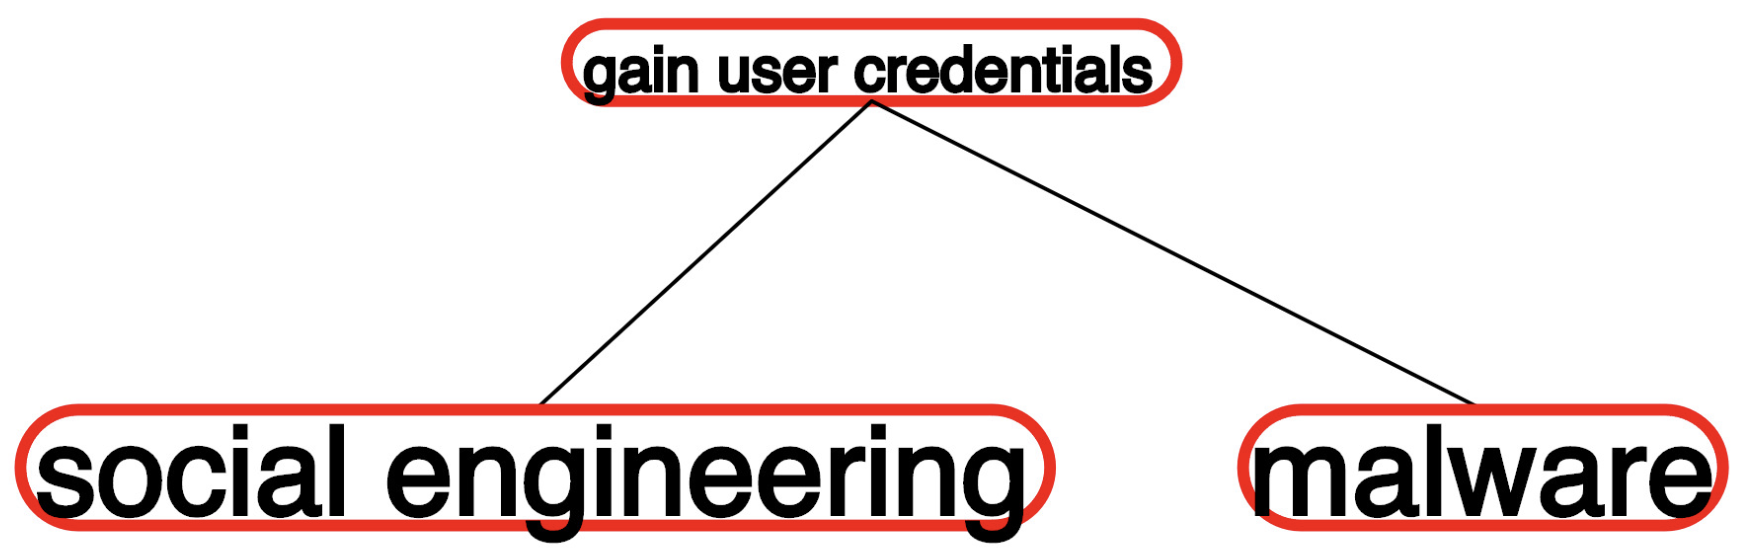
\includegraphics[width=\linewidth]{img/NodeFlip2.png}
%     \end{subfigure}
%     \caption{Two attack trees (subtrees of the example in Figure~\ref{fig:tartgetAT}) with identical information but different node order. These trees would evaluate to have a distance of 2 (two replacement operations).}
%     \label{fig:nodeflipping}
% \end{figure}

% Attack trees, by virtue of their construction, tend to be organized in levels of abstraction. That is, with each new level of an attack tree, the nodes are given to be more specific than the nodes in the previous level. This is shown in Figure~\ref{fig:tartgetAT}, where the root node is given to be the most abstract (as the overall goal), while the leaf nodes are the most concrete (as the individual actions). From this, we find siblings in an attack tree to be on the same level of abstraction. As such, the order of siblings can be changed without affecting the meaning of the attack tree. By checking the order of sibling sets between the two attack trees



% \begin{algorithm}
%     \caption{An algorithm to reorder siblings based on semantic similarity}
%     \label{alg:sibling_reorder}
%     \begin{algorithmic}
%         \State Two attack trees $T_1$ and $T_2$ according to Definition~\ref{def:attack-tree} with $a$ and $b$ total nodes respectively
%         \State $M$ is the mapping of nodes between $T_1$ and $T_2$ \Comment{We give $m[0]$ and $m[1]$ to be the source and target nodes of a mapping for $m \in M$}
%         \State $M \gets T_1[a]\mapsto T_2[b]$\Comment{Root nodes are always mapped}
%         \For{$m \in M$}

%         \State $D \gets []$ \Comment{Matrix of semantic similarity values}
%         \For{left-wise index $i$ in $m[0].\text{children}$}
%         \For{leftwise index $j$ in $m[1].\text{children}$}
%         \State $D[i][j] \gets$
%         \State$\text{  }\text{  }\text{  }\text{  }\text{  }\text{  }\text{  }\text{  }\text{  }\delta(m[0].\text{children}[i].\text{label}, m[1].\text{children}[j].\text{label})$
%         \EndFor
%         \EndFor
%         \State $M_t \gets \emptyset$ \Comment{Temporary set of mappings}
%         \While{$D$ is not empty}
%         \State $i, j \gets \text{argmax}(D)$ \Comment{Largest value in $D$}
%         \State $M_t \gets M_t \cup m[0].\text{children}[i]\mapsto m[1].\text{children}[j]$
%         \State $D \gets D - i$ \Comment{Remove row $i$}
%         \State $D \gets D - j$ \Comment{Remove column $j$}
%         \EndWhile
%         \For{$p$ in $M_t$}
%         \If{indicies $i$, $j$ of $p$ are not equal}
%         \State{Swap nodes $i$ and $j$ \textbf{in $T_1$}}
%         \EndIf
%         \EndFor
%         \State $M \gets M \cup M_t$
%         \EndFor
%     \end{algorithmic}
% \end{algorithm}




\subsection{Radical Distance (RD)}
\label{ssec:rd}

In previous work on attack trees, a proposed mechanism of attack tree decomposition focused on the concept of radicals, or subtrees consisting of a single parent, refinement, and set of children~\cite{schiele2021novel}. We take this decomposition and compare the resulting set of radicals. We define the distance between the resulting radicals according to Algorithm~\ref{alg:recursive-radical} in Appendix~\ref{appendix:alg:radical-distance}.

In Radical Distance (RD), we first decompose into a collection of subtrees that are each a single height, indexed by each subtree's root node. We then perform a semantic comparison of each of the subtree roots, finding a semantic mapping similar to the one discussed for label distance in Section~\ref{ssec:label-distance}. We then calculate the distance subtree by subtree, adding a distance of 1 if the root nodes are not equal, and a distance of 0.5 if the refinements are not equal. For the children, we perform an operation very similar to label distance, but we do not add distance to our calculation if one of the children is already present as a key of the radical dictionaries, as this would result in double counting of that child. This repeats until all children are compared, added, or removed.

As RD is additive, it will always be positive. RD only results in a distance of 0 if the radical roots, refinement, and all child nodes are equal. As the node comparisons use the same mechanism as LD, the node comparisons fulfill the triangle inequality for RD. The refinement comparisons further fulfill the triangle inequality, as either all refinements are the same resulting in an added distance of 0, or a refinement must be changed twice, which would result in a distance of 1. As such, RD fulfills the triangle inequality and is therefore a metric.

% RD as we have defined it does not contain a mechanism to enable tracking of modifications unlike tree edit distance. Unlike label distance however, the full structure of the tree is taken into account. Just as almost all distances we have proposed, our distance does account for the semantic difference between node labels. As RD is 

Applying RD to the examples provided in Figure~\ref{fig:dist-example}, we first compute the radical decomposition of both attack trees. These are the one height subtrees rooted at ``Gain Access'' and ``Phishing'' for Figure~\ref{fig:dist-example-1} and ``Gain Unauthorized Access'' and ``Phishing'' for Figure~\ref{fig:dist-example-2}. We then compute the semantic distance between the root nodes of each of the radicals, in a manner similar to LD, taking the most closely related radicals first. In this case, the two radical roots that are identical (``Phishing'') are selected first, and the radical distance is calculated by comparing the root nodes, refinements, and all children (excluding children that themselves are roots of other radicals). In this case, this comparison yields a difference of 0 given a reasonable value of $\epsilon$. This is repeated for the other two radicals, which have a distance of 1 (``brute force''), resulting in an overall distance of 1 (normalized to 0.167).


\subsection{Multiset Difference (MSD)}
\label{ssec:msd}

Attack trees can be represented mathematically in many different ways. Multiple different representations of attack trees have been proposed, one well-established attack tree semantics is the multiset semantics proposed by Mauw and Oostdijk~\cite{mauw_foundations_2006}. In the multiset semantics, each multiset represents a single complete attack vector within the attack tree. A multiset consisting of multisets represents a node with multiple children. For defining multiset difference, we can use the Jaccard distance between two multisets. However, if we were to use this method, we would need node labels in order for the elements to be considered identical.

If we want to expand the Jaccard distance to count similar-meaning elements of multisets as identical, we would need to calculate the semantic similarity between the elements of the multisets. This would result in a similar problem to the label distance problem or the modification of Zhang and Shasha tree edit distance, as we would need to define a threshold $\epsilon$ for the semantic similarity between two elements. This would result in the same threshold problem as described in Section~\ref{sssec:threshold-problem}, but allow for the multiset distance to account for similar meanings but not identical labels. Ultimately, this results in a calculation that is functionally a nested Jaccard distance, which for reasons similar to LD, means that MSD is a metric~\cite{kosub2019note}.

Multiset semantics, like many mathematical attack tree semantics \cite{jhawar_attack_2015,mauw_foundations_2006}, contain only the leaf node labels. All other labels are reduced from the tree. Additionally, the exact structure of the tree is not generally reconstructible. Ultimately, semantics are meant to answer the question of if two trees are equivalent, which would mean that the exact structure of the tree is not necessarily important. In tree distance, however, the exact structure may be important. By comparing the differences between multisets, we lose some information about the structure of the tree. We also lose the information contained in any intermediate nodes within the tree.

Applying MSD to the examples provided in Figure~\ref{fig:dist-example}, we first calculate the multiset semantic representations of both trees. These semantics would be $\{\{\text{Send Email},$ $\text{Recieve Credentials},\},$ $\{\text{Find unlocked computer}\}\}$ for Figure~\ref{fig:dist-example-1} and $\{\{\text{Send Phishing Email}, \text{Get Credentials}\},$ $\{\text{Find open computer}\},$ $\{\text{Brute force}\}\}$ for Figure~\ref{fig:dist-example-2}. We then calculate the Jaccard distance between each possible pair of sets, using semantic similarity to determine the equivalence of the elements in each set. Starting from the pair of sets with the lowest Jaccard distance (the sets $\{\text{Find unlocked computer}\}$ and $\{\text{Find open computer}\}$), we add the Jaccard distance of these sets (in this case 0) to the overall distance measure. These sets are then removed from the list of sets. This is repeated until all sets are compared, and any sets remaining (in this case $\{\text{Brute force}\}$) are compared to an empty set. In this case, this yields a distance of 1 (normalized to be 0.167) for a reasonable value of $\epsilon$.



\subsection{Weighted Sum Distance (WSD)}
\label{ssec:wsd}

This is a weighted average of the distance approaches discussed above. We will validate and asses the four distance measures described in this section according to our experimental design described in Section~\ref{sec:methodology}. We will then attempt to propose a single distance measure that is the weighted sum of the other four distance measures. This weighted sum can be expressed as the following:
\[
    \alpha_1*\text{LD}+ \alpha_2*\text{TED} + \alpha_3*\text{RD} + \alpha_4*\text{MSD}
\]

For a given vector $\alpha = [\alpha_1, \alpha_2, \alpha_3, \alpha_4]$. We will attempt to provide an optimal alpha such that the performance of this weighted sum outperforms any individual distance measure shown above. As WSD is a sum of metrics, WSD is itself a metric.

Applying WSD to the examples provided in Figure~\ref{fig:dist-example}, we would first calculate LD, TED, RD, and MSD for the two trees. We would then calculate the weighted sum of these values according to the selected value of $\alpha$ to find the WSD. The value of WSD will depend both on the value of $\epsilon$ (as it will affect the four primary distance measures) as well as the selected values of $\alpha$, which affect the sum.

% \subsection{Tree Embedding Distance}

% \NS{I can't find a good way to do this - I could simulate this by combinding BFS position data with the label semantic embeddings, but I dunno if this is a good option}
% Algorithm 2 An algorithm to reorder siblings based on semantic
% similarity



\section{Methodology}
\label{sec:methodology}

We apply the validation methodology described in Section~\ref{sec:validation}.


\subsection{Theoretical Validation}
\label{ssec:methodology-examples}


Outside of the real-world experiment we developed to test the attack tree distance measurements, we also examine the distances measures with a series of theoretical examples. For these basic transformation examples (BTEs), we are not concerned with the semantic similarity,  as this is assessed in our experiment. As such, all labels are single capital letters and we set the similar limit ($\epsilon$) to 1, which would require node to be equivalent in order to be matched.

Each of these examples are simple enough that we can intuitively describe a distance. From this, we can examine how each of our distance measures handle each case. If a distance measure differs significantly from what we expect, this is indicative of the measure being deficient in measure some aspect of the distance between attack trees. The examples are shown in Figure~\ref{fig:counterexamples}.


\newcommand{\CEWidth}{.45\linewidth}
\begin{figure}
    \centering
\begin{subfigure}[b]{\linewidth}
        \centering
        \resizebox{2cm}{!}{
            \begin{forest}
    for tree={
    draw,
    minimum height=.25cm,
    anchor=parent,
    align=center,
    child anchor=parent,
    edge=-
    },
    adnode/.style={rounded rectangle,},
    [{R}, adnode,
            [{I}, adnode,  [{A}, adnode,] [{B}, adnode,]]
                [{J}, adnode, angle below, [{C}, adnode,] [{D}, adnode,]]
        ]
\end{forest}
        }
        \subcaption{Base Attack Tree}\label{sfig:base}
    \end{subfigure}
\begin{subfigure}[b]{\CEWidth}
        \centering
        \resizebox{2cm}{!}{
            \begin{forest}
        for tree={
        draw,
        minimum height=.25cm,
        anchor=parent,
        align=center,
        child anchor=parent,
        edge=-
        },
        adnode/.style={rounded rectangle,},
        [{R}, adnode,
                        [{J}, adnode, angle below, [{D}, adnode,] [{C}, adnode,]]
                                [{I}, adnode,  [{B}, adnode,] [{A}, adnode,]]
                ]
\end{forest}
        }
        \subcaption{Order Reversed}\label{fig:b}
    \end{subfigure}
\begin{subfigure}[b]{\CEWidth}
        \centering
        \resizebox{2cm}{!}{
            \begin{forest}
        for tree={
        draw,
        minimum height=.25cm,
        anchor=parent,
        align=center,
        child anchor=parent,
        edge=-
        },
        adnode/.style={rounded rectangle,},
        [{R}, adnode,
                        [{I}, adnode,  angle below, [{A}, adnode,] [{B}, adnode,]]
                                [{J}, adnode,  [{C}, adnode,] [{D}, adnode,]]
                ]
\end{forest}
        }
        \subcaption{Refinements Switched}\label{fig:b}
    \end{subfigure}
\begin{subfigure}[b]{\CEWidth}
        \centering
        \resizebox{2cm}{!}{
            \begin{forest}
        for tree={
        draw,
        minimum height=.25cm,
        anchor=parent,
        align=center,
        child anchor=parent,
        edge=-
        },
        adnode/.style={rounded rectangle,},
        [{R}, adnode,
                        [{I}, adnode, [{I}, adnode,  [{A}, adnode,] [{B}, adnode,]]]
                                [{K}, adnode]
                                [{J}, adnode, angle below, [{C}, adnode,] [{D}, adnode,]]
                ]
\end{forest}
        }
        \subcaption{Extra Intermediate}\label{fig:b}
    \end{subfigure}
\begin{subfigure}[b]{\CEWidth}
        \centering
        \resizebox{2cm}{!}{
            \begin{forest}
        for tree={
        draw,
        minimum height=.25cm,
        anchor=parent,
        align=center,
        child anchor=parent,
        edge=-
        },
        adnode/.style={rounded rectangle,},
        [{R}, adnode, [{A}, adnode,] [{B}, adnode,]
                                [{J}, adnode, angle below, [{C}, adnode,] [{D}, adnode,]]
                ]
\end{forest}
        }
        \subcaption{Missing Intermediate}\label{fig:b}
    \end{subfigure}
\begin{subfigure}[b]{\CEWidth}
        \centering
        \resizebox{2.5cm}{!}{
            \begin{forest}
        for tree={
        draw,
        minimum height=.25cm,
        anchor=parent,
        align=center,
        child anchor=parent,
        edge=-
        },
        adnode/.style={rounded rectangle,},
        [{R}, adnode,
                        [{I}, adnode,  [{A}, adnode,] [{B}, adnode,][{E}, adnode,]]
                                [{J}, adnode, angle below, [{C}, adnode,] [{D}, adnode,]]
                ]
\end{forest}
        }
        \subcaption{Extra Leaf}\label{fig:b}
    \end{subfigure}
\begin{subfigure}[b]{\CEWidth}
        \centering
        \resizebox{2cm}{!}{
            \begin{forest}
        for tree={
        draw,
        minimum height=.25cm,
        anchor=parent,
        align=center,
        child anchor=parent,
        edge=-
        },
        adnode/.style={rounded rectangle,},
        [{R}, adnode,
                        [{I}, adnode,  [{A}, adnode,] ]
                                [{J}, adnode, angle below, [{C}, adnode,] [{D}, adnode,]]
                ]
\end{forest}
        }
        \subcaption{MissingLeaf}\label{fig:b}
    \end{subfigure}
\begin{subfigure}[b]{\CEWidth}
        \centering
        \resizebox{2cm}{!}{
            \begin{forest}
        for tree={
        draw,
        minimum height=.25cm,
        anchor=parent,
        align=center,
        child anchor=parent,
        edge=-
        },
        adnode/.style={rounded rectangle,},
        [{Z}, adnode,
                        [{I}, adnode,  [{A}, adnode,] [{B}, adnode,]]
                                [{J}, adnode, angle below, [{C}, adnode,] [{D}, adnode,]]
                ]
\end{forest}
        }
        \subcaption{Changed Root}\label{fig:b}
    \end{subfigure}
\begin{subfigure}[b]{\CEWidth}
        \centering
        \resizebox{2cm}{!}{
            \begin{forest}
        for tree={
        draw,
        minimum height=.25cm,
        anchor=parent,
        align=center,
        child anchor=parent,
        edge=-
        },
        adnode/.style={rounded rectangle,},
        [{R}, adnode,
                        [{K}, adnode,  [{A}, adnode,] [{B}, adnode,]]
                                [{J}, adnode, angle below, [{C}, adnode,] [{D}, adnode,]]
                ]
\end{forest}
        }
        \subcaption{Changed Intermediate}\label{fig:b}
    \end{subfigure}
\begin{subfigure}[b]{\CEWidth}
        \centering
        \resizebox{2cm}{!}{
            \begin{forest}
        for tree={
        draw,
        minimum height=.25cm,
        anchor=parent,
        align=center,
        child anchor=parent,
        edge=-
        },
        adnode/.style={rounded rectangle,},
        [{R}, adnode,
                        [{I}, adnode,  [{E}, adnode,] [{B}, adnode,]]
                                [{J}, adnode, angle below, [{C}, adnode,] [{D}, adnode,]]
                ]
\end{forest}
        }
        \subcaption{Changed Leaf}\label{fig:b}
    \end{subfigure}
\begin{subfigure}[b]{\CEWidth}
        \centering
        \resizebox{2cm}{!}{
            \begin{forest}
        for tree={
        draw,
        minimum height=.25cm,
        anchor=parent,
        align=center,
        child anchor=parent,
        edge=-
        },
        adnode/.style={rounded rectangle,},
        [{R}, adnode,
                        [{I}, adnode,  [{A}, adnode,] ]
                                [{J}, adnode, angle below, [{B}, adnode,][{C}, adnode,] [{D}, adnode,]]
                ]
\end{forest}
        }
        \subcaption{Move Adjacent}\label{fig:b}
    \end{subfigure}
\begin{subfigure}[b]{\CEWidth}
        \centering
        \resizebox{2cm}{!}{
            \begin{forest}
        for tree={
        draw,
        minimum height=.25cm,
        anchor=parent,
        align=center,
        child anchor=parent,
        edge=-
        },
        adnode/.style={rounded rectangle,},
        [{R}, adnode,
                        [{I}, adnode,  [{A}, adnode,] ]
                                [{B}, adnode,]
                                [{J}, adnode, angle below, [{C}, adnode,] [{D}, adnode,]]
                ]
\end{forest}
        }
        \subcaption{Move Up}\label{fig:b}
    \end{subfigure}
\begin{subfigure}[b]{\CEWidth}
        \centering
        \resizebox{1.8cm}{!}{
            \begin{forest}
        for tree={
        draw,
        minimum height=.25cm,
        anchor=parent,
        align=center,
        child anchor=parent,
        edge=-
        },
        adnode/.style={rounded rectangle,},
        [{R}, adnode,
                        [{I}, adnode,  [{A}, adnode,[{B}, adnode,]] ]
                                [{J}, adnode, angle below, [{C}, adnode,] [{D}, adnode,]]
                ]
\end{forest}
        }
        \subcaption{Move Down}\label{fig:b}
    \end{subfigure}
\caption{Basic Transformation Examples (BTEs)}\label{fig:counterexamples}
\end{figure}





\subsection{Experimental Validation}

\subsubsection{Experimental Study Design}
\label{ssec:method-study-design}

Students were assigned a project related to attack defense trees as a part of their regular coursework. The project was a mandatory, graded assignment. Students had the option to provide consent for their anonymized responses to be collected for research purposes, this is described in detail in Section~\ref{ssec:ethics}. The assignment consisted of four components. In each component, students were required to create an attack (defense) tree (ADT) using a web application of our own design. Of the four components, the third was included in the assignment for the purposes of validating our approach. The text of the entire study is included in Appendix~\ref{app:exp-questions}; however, we only expound upon the relevant section in this work.

The third component of the study contains two parts. In part A, students were tasked with creating an AT from a provided, written, scenario. The scenario was adapted from an attack tree shown in Naik~\etal~\cite{naikEvaluationPotentialAttack2022}. The scenario was as follows:

\texttt{Many attackers aim to obtain personal data. Gathering personal data can be completed through unauthorized access to profile, credential creep, or a background data attack. Unauthorized access to profile requires gaining user credentials and accessing the profile. The credentials can be gained through a malware attack or a social engineering attack, and the profile can be accessed by stealing a phone or by remote access. Credential creep can be completed by submitting a request for additional data other than what is needed for verification or by user profiling. Finally, a background data attack requires both obtaining a sensitive dataset and linking the dataset via a request for verification.}

This description was created by reading the attack tree in Naik~\etal\ abstraction level by abstraction level, always going from left to right~\cite{naikEvaluationPotentialAttack2022}. The intention of Part A was to assess the requirements of unfiltered labels as well as processing the structure of the attack tree, as the underlying information in the attack trees should be identical between students. As the trees were effectively the same tree, distance between them would more likely be due to an artifact of the distance measure as opposed to the actual distance present in the data. By examining this, we would be able to validate our approach.

We then asked students in part B to expand upon their attack tree by ``doing your own research, add at least 5 new nodes and 2 new refinements to the attack tree you created in the previous section''. In all, this creates a relatively predictable, yet varied, dataset. In Part A, all trees should roughly be the same, baring minor changes in the label of nodes or the order of nodes. We expect that any large differences in part A to be due to misunderstanding the assignment or misreading the scenario. As Part B is built from each students' part A, we expect that the ``core'' of their attack tree to remain unchanged but the added nodes and refinement should introduce an ability to evaluate edit distance. Based on previous experience with similar studies, we expect most students to add exactly 5 new nodes and 2 new refinements, which should allows for some predictable edit distance (namely, the cost of adding 5 new nodes). This allows us to evaluate the distance measures as a metric, as well as further validation. As each student produced two trees, a base and an extension, by comparing them we can validate the distance measures. As if the distance measures are not able to recognize the base tree, the distance measure may not be suitable.

\subsubsection{Analysis}
\label{ssec:method-analysis}
From the first task (AT1), we would expect all trees to be roughly equal. There may be some variation due to missing or added information, from participants who may have deviated from the instructions. We would expect for the average distance of all AT1 trees to remain the same for increasing values of $\epsilon$. From this, we can establish ideal values of $\epsilon$, as once the average distance starts increasing, values that were previously equivalent and likely should be equivalent will start to rise. We can further validate by comparing AT1 to AT2 per participant, as these graphs should be constant for any value of $\epsilon$, as the only difference should be added nodes and added nodes are unaffected by the semantic similarity limit (as added nodes will always have a distance of 1). If the distance measures comparing AT1 to AT2 are not constant for all values of $\epsilon$, this would indicate a distance measure that behaves in an unexpected and potentially invalid manner. Finally, by comparing the difference distance measures on AT2, which are truly different attack trees, we can see if the distance measures behave similarly. Ideally, distance measures incorporate all aspects of attack trees, so their behavior should be similar. If the distance measures do not behave similarly, it may be a sign of an invalid distance measure. Our code for all distance algorithms and analysis is provided here: \url{https://anonymous.4open.science/r/ATD-FB1F/README.md}.

\paragraph{Web Application}

For this assignment, we created a web application which can be used to create attack defense trees. The web application contains a graphic interface with which users can add, delete and modify nodes~\cite{mohalaiaImplementingUserInterface2023}. Additionally, the web application contains an SQL-like language that can be used to generate ADTs~\cite{mezaADTLangDeclarativeLanguage2023}. The Web application additionally allows users to download ADTs as images as well as in the ADTool XML schema as defined by Kordy~\etal~\cite{kordy_adtool_2013}. The web application can be found here: \url{https://anonymous.4open.science/w/ADT-Web-App-AB3C/}.

\subsubsection{Participants}
The participants in this study were all third year bachelor students taking part in a minor on cyber security and governance. Most students were in policy related majors such as Security Studies or International Relations. The participants on average had only a few months of programming experience, which was a result of another course in the minor. Students were asked if they had any prior knowledge of threat models or attack trees, and only a few students had any prior knowledge. Students took this course in the fall semester of 2023. As shown by Naiakshina~\etal\ and Karpati~\etal, in the context of cyber security, students are a sufficient proxy for practitioners~\cite{karpatiComparingAttackTrees2014, naiakshinaConductingSecurityDeveloper2020}.



% \subsubsection{Processing}

% The attack tree data was collected in the form of XML data. This data was then processed using a Python script. The script was used to extract the attack trees from the XML data and to convert the attack trees into a format that could be used by our implementation of the Zhang and Shasha algorithm. We started with the pre-implemented and tested \texttt{zss} library from Tim Henderson~\cite{hendersonZssTreeEdit}. We then modified the library to include our semantic label replacement cost and refinement change cost to create an implementation of the Zhang and Shasha algorithm that should be effective for attack trees. We subsequently used this implementation to calculate the tree edit distance between the attacks trees.  

% Our code for all distance algorithms is provided here: \url{https://anonymous.4open.science/r/ATD-FB1F/README.md}.


\subsubsection{Sentence Embeddings}
\label{ssec:method-embeddings}

As we discussed in Section~\ref{sssec:semantic-similarity}, BERT is a state-of-the-art method for creating sentence embeddings. We use the \texttt{SentenceTransformers} library to calculate the sentence embeddings and cosine similarity to calculate embedding vector difference. As stated previously, our contribution is not the creation of these embeddings; additionally, our use of sentence embeddings is method agnostic, and any method for generating sentence or word embeddings could be used with our methodology. We used multiple different pre-trained BERT models and aggregated the results to illustrate that any results we found were not the result of the use of a specific model. Additionally, we did not fine tune any model. We used the following models: \texttt{paraphrase-multilingual-MiniLM-L12}, \texttt{all-mpnet-base}, and \texttt{all-MiniLM-L12}.

\subsubsection{Ethics}
\label{ssec:ethics}
This study was approved by the the Ethics Review Board at a european university\anonfoot. Students were informed of study and were requested to give consent for their responses to be included in the study. Multiple safeguards were used to ensure that students did not feel pressured into giving consent, as the assignment was a mandatory course component. Students were informed that they could withdraw their consent at any time, and that their responses would be anonymized. 







\section{Results}

\begin{figure}
    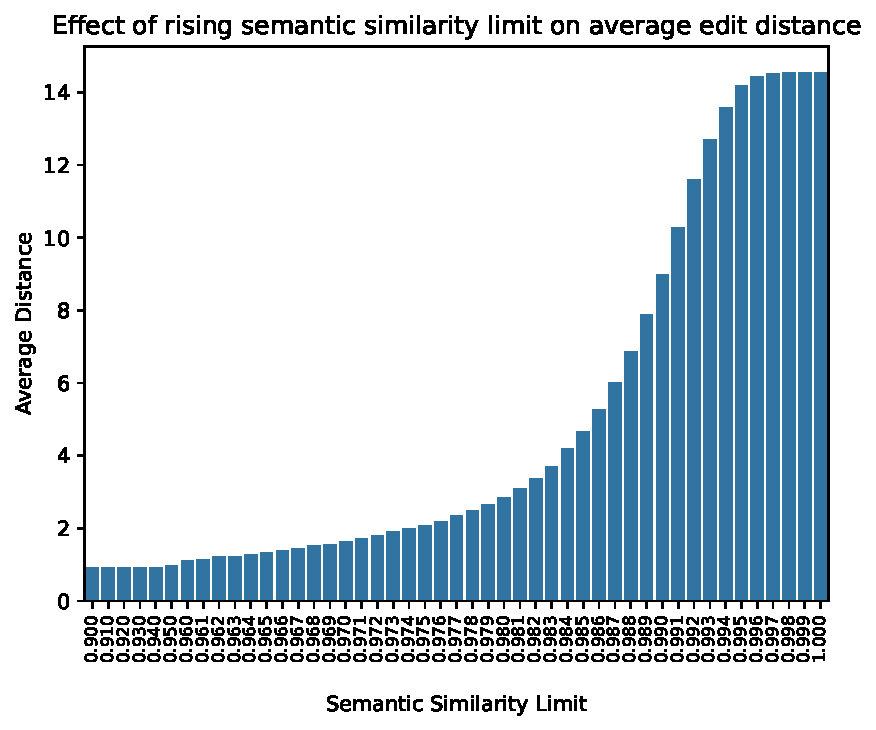
\includegraphics[width=\linewidth]{code/img/similaritylimits.pdf}
\end{figure}

\section{Discussion}
\label{sec:dicsussion}

% RQ1 How can we best calculate the distance between two attack trees?
% RQ2 Is this method of attack tree distance valid?
% RQ3 What are the industry applications of attack tree distance?

\subsection{RQ2: Validity}

To start, we apply tree edit distance, which is a well established and documented mechanism to describe the distance between two trees~\cite{Zhang_Shasha_1989,zhang_editing_1992,akutsu_tree_2021,pawlik_rted_2011,mcvicar_sumoted_2016}. If we can show the distance measures we suggest, label distance, radical distance, and multiset distance, behave similarly to tree edit distance, we can infer that these distance measures are similarly valid. In Figure~\ref{fig:semsim-at2}, we see distance measures for all distance measures as applied to a dataset of trees that all have the same base tree, but have been extended differently by participants. This distance is averaged across all samples we have, and modified by a changing semantic similarity limit. This figure shows how different distance measures change with different semantic similarity limits. This gives us a mechanism to compare different distance measures, as if measures are fundamentally measuring trees similarly, then these lines should roughly correspond to each other. We can see in Figure~\ref{fig:semsim-at2} that the tree edit distance, radical distance and label distance are all remarkably similar, with the lines for these distances translated vertically on the $y$-axis. This suggests that these distance measures are fundamentally measuring the same thing, and as tree edit distance can be argued to be valid, similarly, both label and radical distance must likewise be valid.

Figure~\ref{fig:semsim-at1-2}

Our main contribution to tree distance is the novel technique of comparing components in DAGs by using semantic similarity. To our knowledge, all previous tree distance measurements have worked with either artificial data or with a ``clean'' dataset, which would entirely negate the need to assess node similarity by anything other than equivalence. We are the first to attempt to define tree distance for node labels that are not identical, but should still be considered equivalent. By applying this method to a series of attack trees that should be more or less equivalent, we can assess if this technique is valid. As described in Section~\NS{TODO: Add section reference}, the first attack tree that subjects drew was based on a provided written scenario. Subjects were instructed to include only information provided by the scenario, to include no additional information and to include all the information in the scenario. As such and as discussed in Section~\NS{TODO: Add section reference}, while we expect natural variations in these trees due to participants interpreting the scenario differently, missing information or organizing information different, ultimately the resulting trees should be fairly equivalent. As shown in Figure~\ref{fig:semsim-at1}, for semantic similarity limits  below 0.75, we see this expected equivalence. This suggests that our method is producing an output that is measuring the distance between two attack trees, and thus is valid.

To further validate our approach, we apply our distance measurements


We have shown that our method is able to calculate the distance between two attack trees, and that this distance is valid. We have also shown that this method can be used to compare attack trees in a real-world scenario, and that it can be used to identify similar attack trees.
\section{Conclusion and future work}
\label{sec:conclusion}

Overall, we have proposed several new approaches for defining distance between attack trees, and have offered a comprehensive comparison between those methods. To the best of our knowledge, our work is the first to examine applying the BERT model of semantic embeddings generation to tree distance; further, we are the first to examine tree distance on tree with unfiltered (neither cleaned nor generated) node labels. We have found that traditional tree edit distance applies well with our proposed alterations of semantic similarity to determine node equivalence and an added cost for altering node refinements. Additionally, our proposed distance measure of radical distance is a promising approach for finding distance between trees. We have validated these distance measures and compared them. Finally, we have proposed applications of this research for practical use.

To further this work, we would like to examine the application of semantic similarity to determine node equivalence to potential unordered tree edit distance algorithms. We would also seek to further refine the radical distance measure to better capture the case of tree distance between trees with unequal numbers of radicals. Finally, we would like to apply these distance measures to the problem of automated attack tree generation.

% \cite{*}



\bibliography{bibliography}{}
\bibliographystyle{plain}



\appendix
\section*{Appendix}



\section{Proofs}
\label{appendix:proofs}
\subsection{Proof of Lemma~\ref{lem:gamma-delta}}
\label{appendix:lem:gamma-delta}
\begin{proof}


    \begin{enumerate}
        \item In the case of node removal, there can be no additional cost for changing a refinement. That is, if we remove a node $\ATnode{d}{i}$ from $T$, then we have:

              $$\gamma(\ATnode{d}{i} \rightarrow {\Lambda})$$

              $\Lambda$ is an empty tree, and by definition does not contain any refinements. Therefore, the cost of changing the refinement is zero.

        \item In the case of adding a node, the cost of adding a refinement would be included in the cost of adding the node. That is, if we add a node $\ATnode{d}{i}$ to $T$, then we have:

              $$\gamma(\Lambda \rightarrow {\ATnode{d}{i}})$$

              It is not possible to for a node in an attack tree to not have a refinement. If we separate the cost of adding a node and the cost of adding a refinement, we have one of the two following cases:
              \begin{enumerate}
                  \item A node is added without a refinement, which gives a refinement addition cost of 0, but results in an attack tree which is not valid given our attack tree definition.
                  \item The cost of adding a refinement is \textbf{always} added to the cost of adding a node, which results in the new cost of adding a node to always include $\gamma(\Delta)$.
              \end{enumerate}

              Given one of these cases results in an invalid tree, the other case must always apply. Therefore, by convention, we do not separate the cost of adding a node and the cost of adding a refinement, these are one and the same.

        \item In the case of replacing a node, the cost of replacing a refinement would be:

              $$\gamma({\ATnode{d}{i}} \rightarrow {\ATnode{e}{j}})$$

              Which we declare to consist of the sum following two costs:

              $$\gamma({\ATlabel{d}{i}} \rightarrow {\ATlabel{e}{j}})$$

              Which is the cost of changing one label to another. This is the original cost of replacing a node according to Zhang-Shasha. We also have:

              $$\gamma(\Delta)$$

              Which as previously stated is the cost of changing a refinement.



    \end{enumerate}

\end{proof}

\subsection{Proof of Lemma~\ref{lem:gamma-delta-2}}
\label{appendix:lem:gamma-delta-2}

\begin{proof}
    Let $T$ be an attack tree.

    Assume that $\gamma(\Delta) > \gamma(\ATnode{e}{j} \rightarrow {\Lambda}) + \gamma(\Lambda \rightarrow {\ATnode{e}{j}})$.

    Let $S$ be the optimal sequence of edit operations according to the Zhang-Shasha algorithm. That is, $\gamma(S)$ is minimal for all possible edit sequences for $\delta(T_1, T_2)$ Let some operation $s \in S$ be an operation to replace some node, $\ATnode{d}{i}$, with another, $\ATnode{e}{j}$.

    Thus, $\gamma(s) = \gamma({\ATlabel{d}{i}} \rightarrow {\ATlabel{e}{j}}) + \gamma(\Delta)$

    We have two cases:

    \begin{enumerate}
        \item $\ATnode{d}{i}.\Delta = \ATnode{e}{j}.\Delta$

              In this case, both $\ATnode{d}{i}$ and $\ATnode{e}{j}$ have the same refinement. Thus, $\gamma(\Delta) = 0$. Therefore, $\gamma(s) = \gamma({\ATlabel{d}{i}} \rightarrow {\ATlabel{e}{j}})$.

        \item $\ATnode{d}{i}.\Delta \ne \ATnode{e}{j}.\Delta$

              In this case, both $\ATnode{d}{i}$ and $\ATnode{e}{j}$ have different refinements. Thus, $\gamma(\Delta) > 0$. Therefore, $\gamma(s) = \gamma({\ATlabel{d}{i}} \rightarrow {\ATlabel{e}{j}}) + \gamma(\Delta)$.

              However, we have assumed that $\gamma(\Delta) > \gamma(\ATnode{e}{j} \rightarrow {\Lambda}) + \gamma(\Lambda \rightarrow {\ATnode{e}{j}})$. Therefore, $\gamma(s) = \gamma({\ATlabel{d}{i}} \rightarrow {\ATlabel{e}{j}}) + \gamma(\Delta) > \gamma(\ATnode{e}{j} \rightarrow {\Lambda}) + \gamma(\Lambda \rightarrow {\ATnode{e}{j}})$, as by convention $\gamma$ cannot result in a negative value.

              As such, we can replace $s$ with the sequence of operations $s_1$ and $s_2$, where $s_1$ is the operation to remove $\ATnode{d}{i}$ and $s_2$ is the operation to add $\ATnode{e}{j}$. Thus, $\gamma(s_1) = \gamma(\ATnode{e}{j} \rightarrow {\Lambda})$ and $\gamma(s_2) = \gamma(\Lambda \rightarrow {\ATnode{e}{j}})$. Therefore, $\gamma(s_1) + \gamma(s_2) < \gamma(s)$.

              This results in a contradiction, as $S$ is the optimal sequence of edit operations according to the Zhang-Shasha algorithm, it must not be possible to replace any $s \in S$ with an operation, or sequence of operations, with lower cost.
    \end{enumerate}

    Therefore, if $\gamma(\Delta) > \gamma(\ATnode{e}{j} \rightarrow {\Lambda}) + \gamma(\Lambda \rightarrow {\ATnode{e}{j}})$, then $\gamma(\Delta)$ either must be 0 for a change node edit operation to be included in the optimal sequence of edit operations (case 1), or the optimal sequence of edit operations must always result in node removal then replacement (case 2). In both cases, $\gamma(\Delta)$ is not used.

    Therefore, in order to include the cost of changing refinements in the cost of replacing a node, it must be the case that $\gamma(\Delta) \le \gamma(\ATnode{e}{j} \rightarrow {\Lambda}) + \gamma(\Lambda \rightarrow {\ATnode{e}{j}})$.


\end{proof}



























\section{Experiment Questions}
\label{app:exp-questions}


% \subsection*{ADT 1: Assembling ADTs}

% The following attack \textbf{leaf} nodes are provided. The overall goal of this scenario (and thus the root node of the tree) is \textbf{Rob bank}. Assemble an attack-defense tree using these leaf nodes. Do not add any additional leaf nodes. You may add any intermediary nodes you wish.

% \textbf{Attack leaf nodes:}
% % Why the fuck is there so much space here?
% % \vspace{-10cm}
% % \begin{itemize}
% %   \item Hire Outright
% %   \item Promise part of the stolen money
% %   \item Threaten insiders

% %   \item Buy tools
% %   \item Steal tools
% %   \item Gain Access
% %   \item Walk through front door
% %   \item Locate start of tunnel
% %   \item Find direction to tunnel
% % \end{itemize}

% Hire Outright, Promise part of the stolen money, Threaten insiders, Buy tools, Steal tools, Gain Access, Walk through front door, Locate start of tunnel, Find direction to tunnel

% \textbf{Defense leaf nodes:}

% Personnel Risk Management, Check employee financial situation


% \subsection*{Perception Questions}


% \subsubsection*{Likert Questions}
% \begin{itemize}
%   \setlength{\itemindent}{\qIndent}
%   \item[\surveyq{LS-ADT1-L1}] I find the structure of attack tree easy to understand
%   \item[\surveyq{LS-ADT1-L2}] Given all the nodes of an attack tree, it is easy for me to assemble the tree
%   \item[\surveyq{LS-ADT1-L3}] Given only the leaf nodes of an attack tree, it is easy for me to assemble the tree.
%   \item[\surveyq{LS-ADT1-L4}] I would rather define my own intermediary nodes
%   \item[\surveyq{LS-ADT1-L5}] The process of assembling the attack tree helped me better understand the attack scenario.
% \end{itemize}

% \subsubsection*{Short Response Questions}
% \begin{itemize}
%   \setlength{\itemindent}{\qIndent}
%   \item[\surveyq{LS-ADT1-W1}] What did you find most difficult about this task? Why?
%   \item[\surveyq{LS-ADT1-W2}] How did you go about solving this task? What was your methodology?
% \end{itemize}



% \subsection*{ADT 2: Building ADTs}

% The following text scenario is provided for you. Please create a complete attack defense tree \textbf{of this scenario}. \textbf{Do not add extra information that is not in the scenario}. Try to encapsulate the entire scenario with an attack-defense tree (don't leave any aspect of the attack scenario out).

% \emph{Scenario:} 
% The goal is to open a safe. To open the safe, an attacker can pick the lock,
% learn the combination, cut open the safe, or install the safe improperly so
% that he can easily open it later. Some models of safes are such that they cannot be picked, so if this model is used, then an attacker is unable to pick the lock. There are also auditing services to check if safes and other security technology is installed correctly. To learn the combination, the attacker
% either has to find the combination written down or get the combination
% from the safe owner. If the password is such that the safe owner can remember it, then the safe owner would not need to write it down.



% \subsection*{Perception Questions}

% \subsubsection*{Likert Questions}
% \begin{itemize}
%   \setlength{\itemindent}{\qIndent}
%   \item[\surveyq{LS-ADT2-L1}] I prefer reading attack trees to text descriptions of attacks.
%   \item[\surveyq{LS-ADT2-L2}] The process of building the attack tree helped me better understand the attack scenario.
% \end{itemize}

% \subsubsection*{Short Response Questions}
% \begin{itemize}
%   \setlength{\itemindent}{\qIndent}
%   \item[\surveyq{LS-ADT2-W1}] What did you find most difficult about this task? Why?
%   \item[\surveyq{LS-ADT2-W2}] How did you go about building the ADT?\@ What was your methodology?
%   \item[\surveyq{LS-ADT2-W3}] What was the first node you added to your tree?
% \end{itemize}


% \subsection*{ADT 3: Using Attack Trees}
This question is slightly different than the other questions. You need to create attack trees only. \textbf{This means you should NOT use defense nodes at all for this question}. In Part I, raw an attack tree from the provided scenario; \textbf{include all information from the scenario, do not include information that is not in the scenario}. In Part II, add onto the provided attack tree with new nodes and refinements that you find through your own research.

\subsection*{AT1: Attack tree from scenario}

\emph{Scenario:}  Many attackers aim to obtain personal data. Gathering personal data can be completed through unauthorized access to profile, credential creep, or a background data attack. Unauthorized access to profile requires gaining user credentials and accessing the profile. The credentials can be gained through a malware attack or a social engineering attack, and the profile can be accessed by stealing a phone or by remote access. Credential creep can be completed by submitting a request for additional data other than what is needed for verification or by user profiling. Finally, a background data attack requires both obtaining a sensitive dataset and linking the dataset via a request for verification. 


\subsection*{AT2: Finding new attack components}

Doing your own research, add at least 5 new nodes and 2 new refinements to the attack tree you created in the previous section.





\subsection*{Perception Questions}

\subsubsection*{Likert Questions}
\begin{enumerate}
    \setlength{\itemindent}{\qIndent}
  \item[\surveyq{LS-ADT3-L1}] I prefer reading attack trees to text descriptions of attacks.
  \item[\surveyq{LS-ADT3-L2}] The process of building the attack tree helped me better understand the attack scenario.
  \item[\surveyq{LS-ADT3-L3}]  The ADT communicates the attack scenario better than the written scenario.
  \item[\surveyq{LS-ADT3-L4}] Using the ADT Web App made this task easier than if I had done it by hand.
\end{enumerate}

\subsubsection*{Short Response Questions}
\begin{enumerate}
    \setlength{\itemindent}{\qIndent}
  \item[\surveyq{LS-ADT3-W1}] What did you find most difficult about this task? Why?
  \item[\surveyq{LS-ADT3-W2}] How did you go about building the ADT? What was your methodology?
  \item[\surveyq{LS-ADT3-W3}] What was the first node you added to your tree?
  \item[\surveyq{LS-ADT3-W4}]How would you describe using the ADT Web App? What aspects of the app made this task easier? What aspects made this task harder?
\end{enumerate}

% \subsection*{ADT 4: Creating ADTs}

% Construct an attack defense tree of a scenario of your choice. Your tree should be complete (covers all reasonable attack scenarios) and reasonably large.


% \subsection*{Perception Questions}

% \subsubsection*{Likert Questions}
% \begin{itemize}
%   \setlength{\itemindent}{\qIndent}
%   \item[\surveyq{LS-ADT4-L1}] The process of creating the attack tree helped me better understand the attack scenario I selected
%   \item[\surveyq{LS-ADT4-L2}] I feel I could have achieved the same understanding by writing a text description of the attack.
%   \item[\surveyq{LS-ADT4-L3}] The ADT I created would help me communicate my threat scenario.
% \end{itemize}

% \subsubsection*{Short Response Questions}
% \begin{itemize}
%   \setlength{\itemindent}{\qIndent}
%   \item[\surveyq{LS-ADT4-W1}] What did you find easy about using ADTs?
%   \item[\surveyq{LS-ADT4-W2}] What did you find difficult about using ADT?\@
%   \item[\surveyq{LS-ADT4-W3}] Do you think ADTs have a place in the cybersecurity industry? If so, where? If not, why not?
%   \item[\surveyq{LS-ADT4-W4}] What aspects, if any, do you think are missing from ADTs?
%   \item[\surveyq{LS-ADT4-W5}] Do you hope to encounter ADTs in the future?
% \end{itemize}



% \section{Operations table for counterexamples}
\begin{table*}[b!]
  \resizebox{\textwidth}{!}{
      \begin{tabular}{lcccccccccccccccc}
          \toprule
          Counterexample       & \multicolumn{4}{|c|}{Label Distance} & \multicolumn{4}{|c|}{Tree Edit Distance} & \multicolumn{4}{|c|}{Radical Distance} & \multicolumn{4}{|c|}{Multiset Distance}                                                                                                 \\
                               & Remove                               & Add                                      & Change                                 & Match                                   & Remove & Add & Change & Match & Remove & Add & Change & Match & Remove & Add & Change & Match \\
          \midrule
          Order Reversed       & 0                                    & 0                                        & 0                                      & 7                                       & 0      & 0   & 6      & 1     & 0      & 0   & 0      & 7     & 0      & 0   & 0      & 4     \\
          Refinement Switch    & 0                                    & 0                                        & 0                                      & 7                                       & 0      & 0   & 2      & 5     & 0      & 0   & 2      & 5     & 1      & 1   & 1      & 2     \\
          Extra Intermediate   & 1                                    & 0                                        & 0                                      & 7                                       & 1      & 0   & 0      & 7     & 1      & 0   & 0      & 7     & 0      & 0   & 0      & 4     \\
          Missing Intermediate & 0                                    & 1                                        & 0                                      & 6                                       & 0      & 1   & 0      & 6     & 1      & 3   & 0      & 4     & 0      & 0   & 0      & 4     \\
          Extra Leaf           & 1                                    & 0                                        & 0                                      & 7                                       & 1      & 0   & 0      & 7     & 1      & 0   & 0      & 7     & 1      & 0   & 0      & 4     \\
          Missing Leaf         & 0                                    & 1                                        & 0                                      & 6                                       & 0      & 1   & 0      & 6     & 0      & 1   & 0      & 6     & 0      & 1   & 0      & 3     \\
          Changed Root         & 0                                    & 0                                        & 1                                      & 6                                       & 0      & 0   & 1      & 6     & 0      & 0   & 1      & 6     & 0      & 0   & 0      & 4     \\
          Changed Intermediate & 0                                    & 0                                        & 1                                      & 6                                       & 0      & 0   & 1      & 6     & 0      & 0   & 1      & 6     & 0      & 0   & 0      & 4     \\
          Changed Leaf         & 0                                    & 0                                        & 1                                      & 6                                       & 0      & 0   & 1      & 6     & 0      & 0   & 1      & 6     & 0      & 0   & 1      & 3     \\
          Move Adjacent        & 0                                    & 0                                        & 0                                      & 7                                       & 1      & 1   & 0      & 6     & 1      & 1   & 0      & 6     & 1      & 2   & 0      & 2     \\
          Move Up              & 0                                    & 0                                        & 0                                      & 7                                       & 1      & 1   & 0      & 6     & 1      & 1   & 0      & 6     & 0      & 0   & 0      & 4     \\
          Move Down            & 0                                    & 0                                        & 0                                      & 7                                       & 1      & 1   & 0      & 6     & 2      & 1   & 0      & 5     & 0      & 1   & 0      & 3     \\
          \bottomrule
      \end{tabular}

  }
  \caption{Table showing the operations per counterexample and distance measure}
\end{table*}





\section{Algorithms}
\label{appendix:algorithms}

\subsection{Label Distance Algorithm}
\label{appendix:alg:label-distance}
\begin{algorithm}[H]
    \caption{An algorithm to calculate the label distance between two attack trees.}
    \label{alg:label-distance}
    \begin{algorithmic}
        \State Two attack trees $T_1$ and $T_2$ according to Definition~\ref{def:attack-tree} with $a$ and $b$ total nodes respectively
        \State $M$ is the set of mappings between nodes in $T_1$ and $T_2$
        \State $A$ is the list of node labels in $T_1$
        \State $B$ is the list of node labels in $T_2$
        \State $d$ is the distance between attack trees
        \State $M \gets \emptyset$
        \State Let $L$ be the $a \times b$ matrix of semantic similarity values between labels in $A$ and $B$
        \While{$L$ is not empty}
        \State Find the maximum value, $\delta$, in $L$ at index $i, j$
        \State Remove row $i$ and column $j$ from $L$
        \If{$\delta > \epsilon$}
        \State Add $(A[i], B[j], \delta)$ to $M$
        \Else
        \State Add $(A[i], \Lambda, 0)$ to $M$
        \State Add $(\Lambda, B[j], 0)$ to $M$
        \State $d = d + 1$
        \EndIf
        \State Remove $A[i]$ from $A$
        \State Remove $B[j]$ from $B$
        \EndWhile
        \For{each $a \in A$}
        \State Add $(a, \Lambda, 1)$ to $M$
        \State $d = d + 1$
        \EndFor
        \For{each $b \in B$}
        \State Add $(\Lambda, b, 1)$ to $M$
        \State $d = d + 1$
        \EndFor
        \State \Return $d$, $M$
    \end{algorithmic}
\end{algorithm}

\subsection{Radical Distance Algorithm}
\label{appendix:alg:radical-distance}
\begin{algorithm}[H]
    \caption{An algorithm to compute radical distance}
    \label{alg:recursive-radical}
    \begin{algorithmic}
        \State Two attack trees $T_1$ and $T_2$ according to Definition~\ref{def:attack-tree} with $a$ and $b$ total nodes respectively
\State $D_1$, $D_2$ $\gets$ the radical dictionary according to the decomposition in \cite{schiele2021novel} for $T_1$ and $T_2$, respectively
        \State $M$ $\gets$ the mapping between $D_1$ and $D_2$ indexed by radical root nodes according to semantic similarity (from semantic label distance)
        \State $d \gets 0$
        \For{$m \in M$, where $m = (\ATnode{d}{i}, \ATnode{e}{j})$ and $\ATnode{d}{i}, \ATnode{e}{j}$ are indices for $D_1$, and $D_2$, respectively}
        \If {$\delta(\ATnode{d}{i}, \ATnode{e}{j}) < \epsilon$}
        \State $d \gets d + 1$
        \EndIf
        \If {$Delta(\ATnode{d}{i}) \ne Delta(\ATnode{e}{j})$ and $\ATnode{d}{i}, \ATnode{e}{j} \ne \Lambda$}
        \State $d \gets d + 0.5$
        \EndIf
        \State $M_c \gets$ the semantic mappings (from semantic label distance) between child$(\ATnode{d}{i})$ and child$(\ATnode{e}{j})$
        \For{$c \in M_c$ where  $c = (\ATnode{d+1}{p}, \ATnode{e+1}{q})$}
        \If{$\ATnode{d+1}{p} \not\in D_1$ and $\ATnode{e+1}{p} \not\in D_2$
            \If $\delta(\ATnode{d+1}{p}, \ATnode{e+1}{q}) < \epsilon$}
        \State $d \gets d + 1$
        \EndIf
        \EndIf
        \EndFor
        \EndFor
        \State \Return $d$
    \end{algorithmic}
\end{algorithm}









% \appendix
% \input{content/questionnaire}

\end{document}
